%\RequirePackage[l2tabu, orthodox]{nag}
\RequirePackage{currfile}
\documentclass[12pt]{beamer}
\graphicspath{{Imagenes/}{../Imagenes/}}
\usepackage[utf8]{inputenc}
\usepackage[spanish]{babel}
\usepackage{standalone}
\usepackage{color}
\usepackage[binary-units=true]{siunitx}
\usepackage{hyperref}
\hypersetup{
  colorlinks=true,
  linkcolor=blue,          % color of internal links (change box color with linkbordercolor)
  citecolor=green,        % color of links to bibliography
  filecolor=magenta,      % color of file links
  urlcolor=cyan,           % color of external links
  linkbordercolor={0 0 1}
}
\usepackage{xcolor, soul}
\usepackage{etoolbox}
\usepackage{amsmath}
\usepackage{amsthm}
\usepackage{physics}
\usepackage{multicol}
\usepackage{graphicx}
\usepackage{bookmark}
\usepackage{longtable}
\usepackage{graphicx}
\usepackage{tikz}
\usepackage[siunitx, RPvoltages]{circuitikz}
\usetikzlibrary{mindmap}
\usetikzlibrary{arrows, patterns, shapes, decorations.markings, decorations.pathmorphing}
\usetikzlibrary{matrix,positioning}
\tikzstyle{every picture}+=[remember picture,baseline]
\usepackage[autostyle,spanish=mexican]{csquotes}
\usepackage{pifont}
\usepackage[font=footnotesize,textfont=it]{caption}
\usepackage{tabulary}
\usepackage{booktabs}
\usepackage[outdir=./]{epstopdf}
%\usepackage{epstopdf}
\usepackage{media9}
\usepackage{multimedia}
\usepackage{bigints}
%\usepackage{enumitem}
\usepackage[os=win]{menukeys}
\usepackage{pifont}
\usepackage{pbox}
\usepackage{alltt}
\usepackage{verbatim}
\usepackage{colortbl}
\usepackage{tcolorbox}
\usepackage{fancyvrb}
\usepackage[sfdefault]{roboto}  %% Option 'sfdefault' only if the base font of the document is to be sans serif
%\usepackage[T1]{fontenc}
\setcounter{secnumdepth}{3}
\setcounter{tocdepth}{3}
\DeclareGraphicsExtensions{.pdf,.png,.jpg}
\renewcommand {\arraystretch}{1.5}
\definecolor{ao}{rgb}{0.0, 0.5, 0.0}
\definecolor{aquamarine}{rgb}{0.5, 1.0, 0.83}
\definecolor{kellygreen}{rgb}{0.3, 0.73, 0.09}
\definecolor{bisque}{rgb}{1.0, 0.89, 0.77}
\definecolor{amber}{rgb}{1.0, 0.75, 0.0}
\definecolor{armygreen}{rgb}{0.29, 0.33, 0.13}
\definecolor{alizarin}{rgb}{0.82, 0.1, 0.26}
\definecolor{cadetblue}{rgb}{0.37, 0.62, 0.63}
\newcommand*{\TitleParbox}[1]{\parbox[c]{6cm}{\raggedright #1}}%
\newcommand{\python}{\texttt{python}}
\newcommand{\textoazul}[1]{\textcolor{blue}{#1}}
\newcommand{\azulfuerte}[1]{\textcolor{blue}{\textbf{#1}}}
\newcommand{\funcionazul}[1]{\textcolor{blue}{\textbf{\texttt{#1}}}}
%\normalfont
\usepackage{ccfonts}% http://ctan.org/pkg/{ccfonts}
\usepackage[T1]{fontenc}% http://ctan.or/pkg/fontenc
\renewcommand{\rmdefault}{cmr}% cmr = Computer Modern Roman
\usefonttheme[onlymath]{serif}
\linespread{1.3}
\newcounter{saveenumi}
\newcommand{\seti}{\setcounter{saveenumi}{\value{enumi}}}
\newcommand{\conti}{\setcounter{enumi}{\value{saveenumi}}}
\newcommand{\tikzmark}[1]{\tikz[remember picture] \node[coordinate] (#1) {#1};}

\usepackage{scalerel}[2016-12-29]
\def\stretchint#1{\vcenter{\hbox{\stretchto[440]{\displaystyle\int}{#1}}}}
\def\scaleint#1{\vcenter{\hbox{\scaleto[3ex]{\displaystyle\int}{#1}}}}
\def\bs{\mkern-12mu}

\newtheorem{teo}{}[section]
\usepackage{blkarray}

%reduce el tamaño de letra de la etiqueta equations
\makeatletter
\def\maketag@@@#1{\hbox{\m@th\normalfont\small#1}}
\makeatother

%se usa para la x en itemize
\newcommand{\xmark}{\text{\ding{55}}}

%\AtBeginDocument{\setlength{\tymin}{1em}}


\definecolor{myblue}{rgb}{.8, .8, 1}

\usepackage{empheq}

\newlength\mytemplen
\newsavebox\mytempbox

\makeatletter
\newcommand\mybluebox{%
    \@ifnextchar[%]
       {\@mybluebox}%
       {\@mybluebox[0pt]}}

\def\@mybluebox[#1]{%
    \@ifnextchar[%]
       {\@@mybluebox[#1]}%
       {\@@mybluebox[#1][0pt]}}

\def\@@mybluebox[#1][#2]#3{
    \sbox\mytempbox{#3}%
    \mytemplen\ht\mytempbox
    \advance\mytemplen #1\relax
    \ht\mytempbox\mytemplen
    \mytemplen\dp\mytempbox
    \advance\mytemplen #2\relax
    \dp\mytempbox\mytemplen
    \colorbox{myblue}{\hspace{1em}\usebox{\mytempbox}\hspace{1em}}}

\makeatother



%Se usa la plantilla Madrid modificada con beaver
\mode<presentation>
{
  \usetheme{Madrid}
  \setbeamertemplate{headline}{}
  %\useoutertheme{infolines}
  \usecolortheme{beaver}
  \setbeamercovered{invisible}
  

\setbeamertemplate{section in toc}[sections numbered]
\setbeamertemplate{subsection in toc}[subsections numbered]
\setbeamertemplate{subsection in toc}{\leavevmode\leftskip=3.2em\rlap{\hskip-2em\inserttocsectionnumber.\inserttocsubsectionnumber}\inserttocsubsection\par}
\setbeamercolor{section in toc}{fg=blue}
\setbeamercolor{subsection in toc}{fg=blue}
\setbeamerfont{subsection in toc}{size=\small}

\setbeamertemplate{navigation symbols}{}
\setbeamertemplate{caption}[numbered]

}

\usepackage{courier}
\usepackage{listingsutf8}
\usepackage{listings}
\usepackage{xcolor}
\usepackage{textcomp}
\usepackage{color}
\definecolor{deepblue}{rgb}{0,0,0.5}
\definecolor{brown}{rgb}{0.59, 0.29, 0.0}
\definecolor{OliveGreen}{rgb}{0,0.25,0}
% \usepackage{minted}

\DeclareCaptionFont{white}{\color{white}}
\DeclareCaptionFormat{listing}{\colorbox{gray}{\parbox{0.98\textwidth}{#1#2#3}}}
\captionsetup[lstlisting]{format=listing,labelfont=white,textfont=white}
\renewcommand{\lstlistingname}{Código}


\definecolor{Code}{rgb}{0,0,0}
\definecolor{Keywords}{rgb}{255,0,0}
\definecolor{Strings}{rgb}{255,0,255}
\definecolor{Comments}{rgb}{0,0,255}
\definecolor{Numbers}{rgb}{255,128,0}

\makeatletter

\newif\iffirstchar\firstchartrue
\newif\ifstartedbyadigit
\newif\ifprecededbyequalsign

\newcommand\processletter
{%
  \ifnum\lst@mode=\lst@Pmode%
    \iffirstchar%
        \global\startedbyadigitfalse%
      \fi
      \global\firstcharfalse%
    \fi
}

\newcommand\processdigit
{%
  \ifnum\lst@mode=\lst@Pmode%
      \iffirstchar%
        \global\startedbyadigittrue%
      \fi
      \global\firstcharfalse%
  \fi
}

\lst@AddToHook{OutputOther}%
{%
  \lst@IfLastOtherOneOf{=}
    {\global\precededbyequalsigntrue}
    {}%
}

\lst@AddToHook{Output}%
{%
  \ifprecededbyequalsign%
      \ifstartedbyadigit%
        \def\lst@thestyle{\color{orange}}%
      \fi
    \fi
  \global\firstchartrue%
  \global\startedbyadigitfalse%
  \global\precededbyequalsignfalse%
}

\lstset{ 
language=Python,                % choose the language of the code
basicstyle=\footnotesize\ttfamily,       % the size of the fonts that are used for the code
numbers=left,                   % where to put the line-numbers
numberstyle=\scriptsize,      % the size of the fonts that are used for the line-numbers
stepnumber=1,                   % the step between two line-numbers. If it is 1 each line will be numbered
numbersep=5pt,                  % how far the line-numbers are from the code
backgroundcolor=\color{white},  % choose the background color. You must add \usepackage{color}
showspaces=false,               % show spaces adding particular underscores
showstringspaces=false,         % underline spaces within strings
showtabs=false,                 % show tabs within strings adding particular underscores
frame=single,   		% adds a frame around the code
tabsize=2,  		% sets default tabsize to 2 spaces
captionpos=t,   		% sets the caption-position to bottom
breaklines=true,    	% sets automatic line breaking
breakatwhitespace=false,    % sets if automatic breaks should only happen at whitespace
escapeinside={\#},  % if you want to add a comment within your code
stringstyle =\color{OliveGreen},
%otherkeywords={{as}},             % Add keywords here
keywordstyle = \color{blue},
commentstyle = \color{black},
identifierstyle = \color{black},
literate=%
         {á}{{\'a}}1
         {é}{{\'e}}1
         {í}{{\'i}}1
         {ó}{{\'o}}1
         {ú}{{\'u}}1
%
%keywordstyle=\ttb\color{deepblue}
%fancyvrb = true,
}

\lstdefinestyle{FormattedNumber}{%
    literate={0}{{\textcolor{red}{0}}}{1}%
             {1}{{\textcolor{red}{1}}}{1}%
             {2}{{\textcolor{red}{2}}}{1}%
             {3}{{\textcolor{red}{3}}}{1}%
             {4}{{\textcolor{red}{4}}}{1}%
             {5}{{\textcolor{red}{5}}}{1}%
             {6}{{\textcolor{red}{6}}}{1}%
             {7}{{\textcolor{red}{7}}}{1}%
             {8}{{\textcolor{red}{8}}}{1}%
             {9}{{\textcolor{red}{9}}}{1}%
             {.0}{{\textcolor{red}{.0}}}{2}% Following is to ensure that only periods
             {.1}{{\textcolor{red}{.1}}}{2}% followed by a digit are changed.
             {.2}{{\textcolor{red}{.2}}}{2}%
             {.3}{{\textcolor{red}{.3}}}{2}%
             {.4}{{\textcolor{red}{.4}}}{2}%
             {.5}{{\textcolor{red}{.5}}}{2}%
             {.6}{{\textcolor{red}{.6}}}{2}%
             {.7}{{\textcolor{red}{.7}}}{2}%
             {.8}{{\textcolor{red}{.8}}}{2}%
             {.9}{{\textcolor{red}{.9}}}{2}%
             {\ }{{ }}{1}% handle the space
         ,%
          %mathescape=true
          escapeinside={__}
          }



\makeatletter
\setbeamercolor{section in foot}{bg=green!30!cyan, fg=black!90!orange}
\setbeamercolor{subsection in foot}{bg=red!30!cyan, fg=red}
%\setbeamercolor{date in foot}{bg=orange!30!cyan, fg=red}
\setbeamertemplate{footline}
{
  \leavevmode%
  \hbox{%
  \begin{beamercolorbox}[wd=.333333\paperwidth,ht=2.25ex,dp=1ex,center]{section in foot}%
    \usebeamerfont{section in foot} \insertsection
  \end{beamercolorbox}}%
  \begin{beamercolorbox}[wd=.333333\paperwidth,ht=2.25ex,dp=1ex,center]{subsection in foot}%
    \usebeamerfont{subsection in foot}  \insertsubsection
  \end{beamercolorbox}%
  \begin{beamercolorbox}[wd=.333333\paperwidth,ht=2.25ex,dp=1ex,right]{date in head/foot}%
    \usebeamerfont{date in head/foot} \insertshortdate{} \hspace*{2em}
    \insertframenumber{} / \inserttotalframenumber \hspace*{2ex} 
  \end{beamercolorbox}}%
  \vskip0pt%
\makeatother
\title{\large{Tema 2 - Operaciones matemáticas básicas}}
\subtitle{Cálculo de raíces}
\author{M. en C. Gustavo Contreras Mayén}
\date{\today}
\institute{Facultad de Ciencias - UNAM}
\titlegraphic{
\includegraphics[width=1.75cm]{Imagenes/escudo-facultad-ciencias}\hspace*{4.75cm}~%
   
\includegraphics[width=1.75cm]{Imagenes/escudo-unam}
}
\begin{document}
\maketitle
\fontsize{14}{14}\selectfont
\spanishdecimal{.}
\section*{Contenido}
\frame{\tableofcontents[currentsection, hideallsubsections]}
\section{Bases generales}
\frame{\tableofcontents[currentsection, hideothersubsections]}
\subsection{Cálculo de raíces}
\begin{frame}
\frametitle{Cálculo de raíces}
Sea $y= f(x)$.  
\\
\bigskip
Los valores de $x$ que hacen que $y=0$ se denominan \textcolor{blue}{raíces de la ecuación}.
\end{frame}
\begin{frame}
\frametitle{Cálculo de raíces}
El teorema fundamental del álgebra indica que todo polinomio de grado $n$, tiene $n$ raíces.
\\
\bigskip
En el caso de las raíces reales, corresponden a los valores de $x$ que hacen que la función corte el eje de las abscisas:
\end{frame}
\begin{frame}
\frametitle{Ejemplo de la función seno(x)}
\begin{figure}
	\centering
	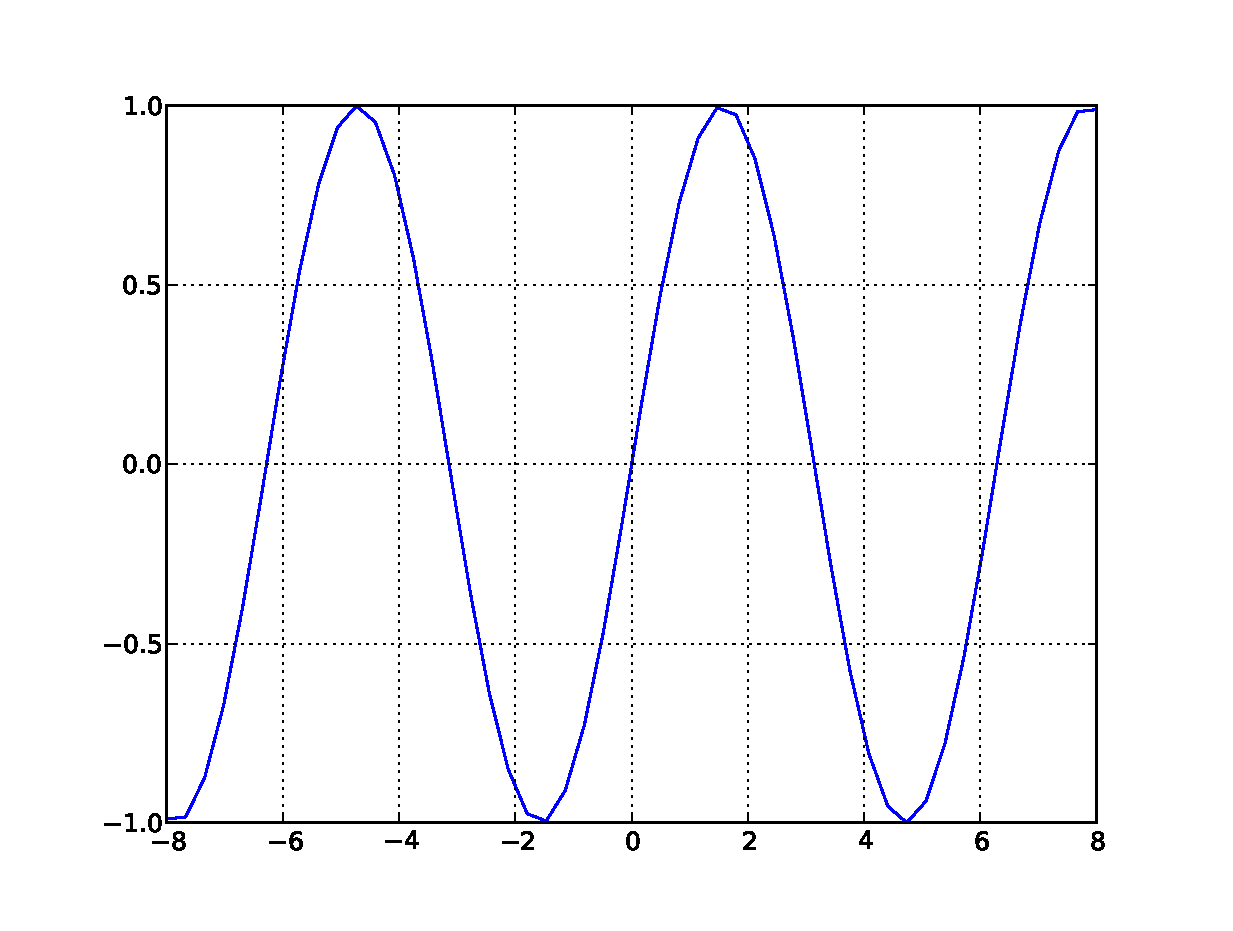
\includegraphics[scale=0.4]{Imagenes/raices00.eps}
	\caption{La función tiene varias raíces en el intervalo.} 
\end{figure}
\end{frame}
\begin{frame}
\frametitle{Tipo de raíces}
Las raíces de un polinomio pueden ser reales o complejas.
\\
\bigskip
Si un polinomio tiene coeficientes reales
\[ a_{0},a_{1},a_{2},\ldots,a_{n-1},a_{n} \]
entonces todas las raíces complejas siempre ocurrirán en pares conjugados complejos.
\end{frame}
\begin{frame}
\frametitle{Tipo de raíces}
Por ejemplo, un polinomio cúbico tiene la siguiente
forma general:
\[ f(x) = a_{0} \: x^{3} + a_{1} \: x^{2} + a_{2} \: x + a_{3}\]
\setbeamercolor{item projected}{bg=purple!70!black,fg=white}
\setbeamertemplate{enumerate items}[circle]
\begin{enumerate}[<+->]
\item Tres raíces reales distintas.
\item Una raíz real con multiplicidad 3.
\item Una raíz real simple y una raíz real con multiplicidad 2.
\item Una raíz real y un par conjugado complejo.
\end{enumerate}
\end{frame}
\begin{frame}[fragile]
\setbeamerfont{caption}{size=\scriptsize}
\captionsetup{justification=centering}
\frametitle{Tres raíces distintas}
\begin{minipage}{5cm}
\fontsize{12}{12}\selectfont
\begin{align*}
f(x) & = x^{3} - 3 \: x^{2} - x + 3 \\
&= (x - 3)(x + 1)(x - 1)
\end{align*}
Las raíces son:
\begin{align*}
x_{1} &= 3 \\
x_{2} &= 1 \\
x_{3} &= -1 \\
\end{align*}
\end{minipage}
\hspace{0.5cm}
\begin{minipage}{4.5cm}
\begin{figure}
	\centering
	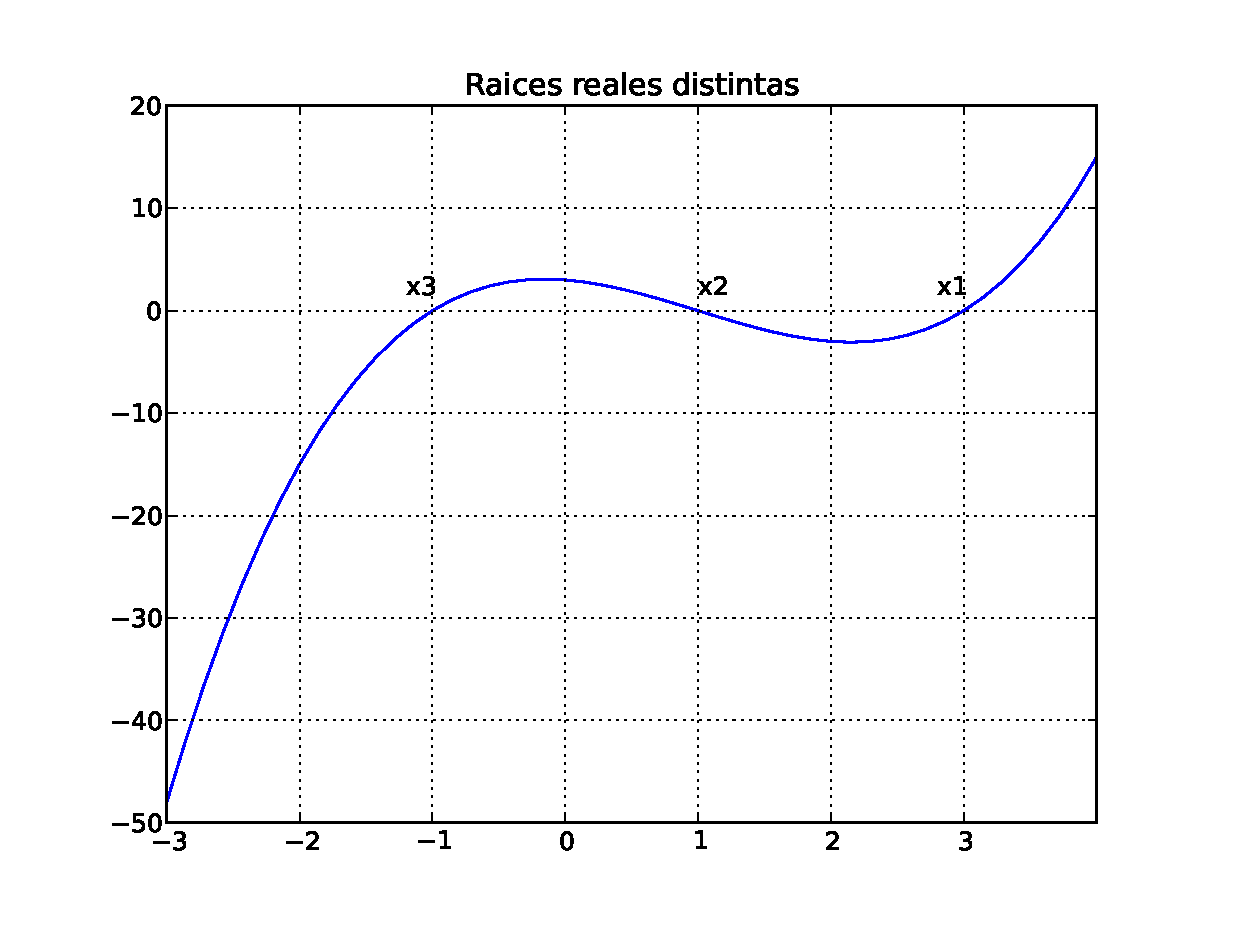
\includegraphics[scale=0.3]{Imagenes/raices01.eps}
	%\vspace{0.5cm}
	\caption{Los valores $x_{i}$ representan las raíces del polinomio.}
\end{figure}
\end{minipage}
\end{frame}
\begin{frame}[fragile]
\setbeamerfont{caption}{size=\scriptsize}
\captionsetup{justification=centering}
\frametitle{Raíz real con multiplicidad 3}
\begin{minipage}{5cm}
\fontsize{12}{12}\selectfont
\begin{align*}
f(x) &=  x^{3} - 6 \: x^{2} + 12 \: x - 8 \\
&= (x - 2)^{3}
\end{align*}
Las raíces son:
\begin{align*}
x_{1} &= 2 \\
x_{2} &= 2 \\
x_{3} &= 2 \\
\end{align*}
\end{minipage}
\hspace{0.5cm}
\begin{minipage}{4.5cm}
\begin{figure}
	\centering
	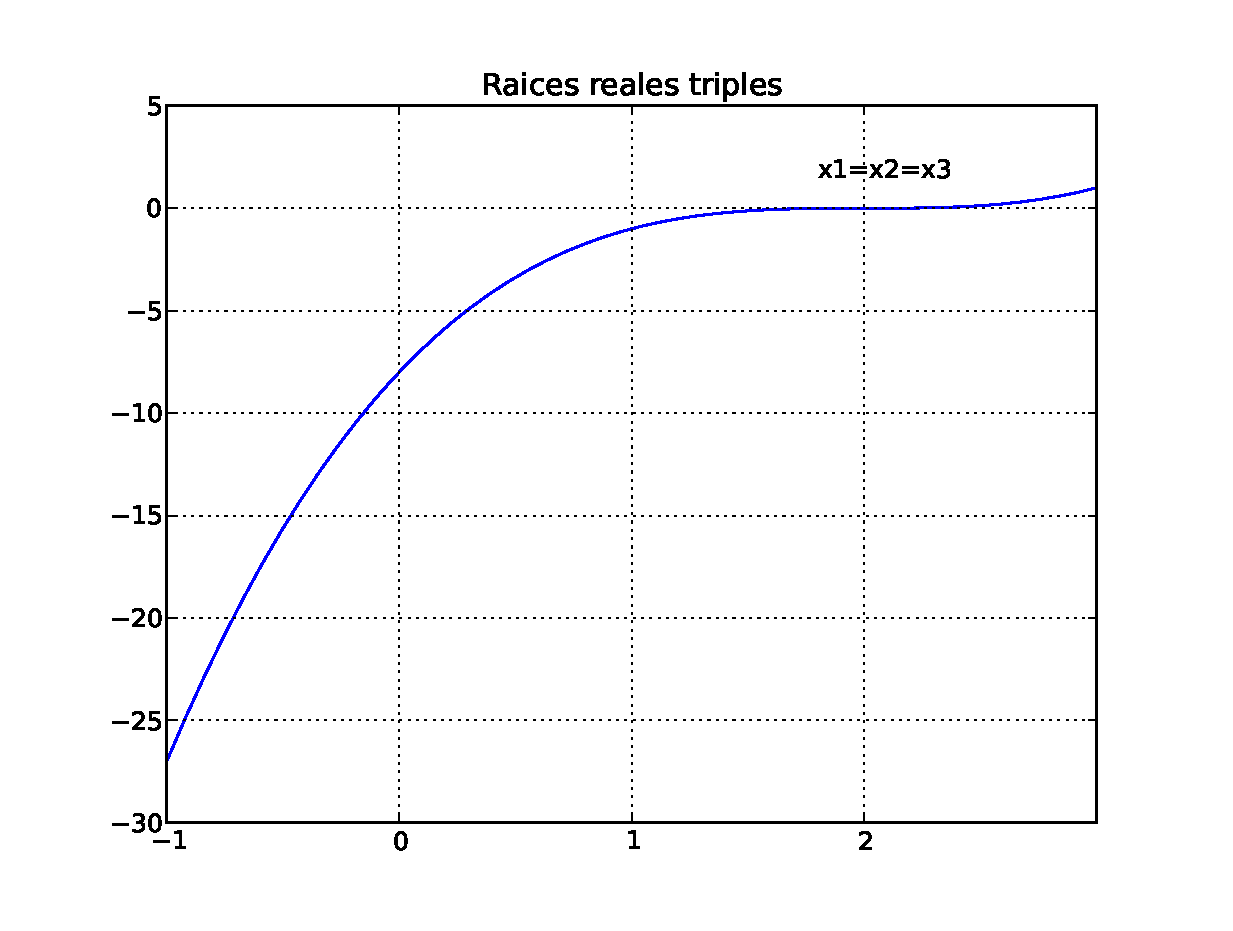
\includegraphics[scale=0.3]{Imagenes/raices02.eps}
	\caption{El valor de las raíces $x_{i}$ coinciden.} 
\end{figure}
\end{minipage}
\end{frame}
\begin{frame}[fragile]
\setbeamerfont{caption}{size=\scriptsize}
\captionsetup{justification=centering}
\frametitle{Raíz real y una raíz real con multiplicidad 2}
\begin{minipage}{5cm}
\fontsize{12}{12}\selectfont
\begin{align*}
f(x) &= x^{3} - 12 \: x + 16 \\
&= (x + 4)(x - 2)^{2}
\end{align*}
Las raíces son:
\begin{align*}
x_{1} &= -4 \\
x_{2} &= 2 \\
x_{3} &= 2 \\
\end{align*}
\end{minipage}
\hspace{0.5cm}
\begin{minipage}{4.5cm}
\begin{figure}
	\centering
	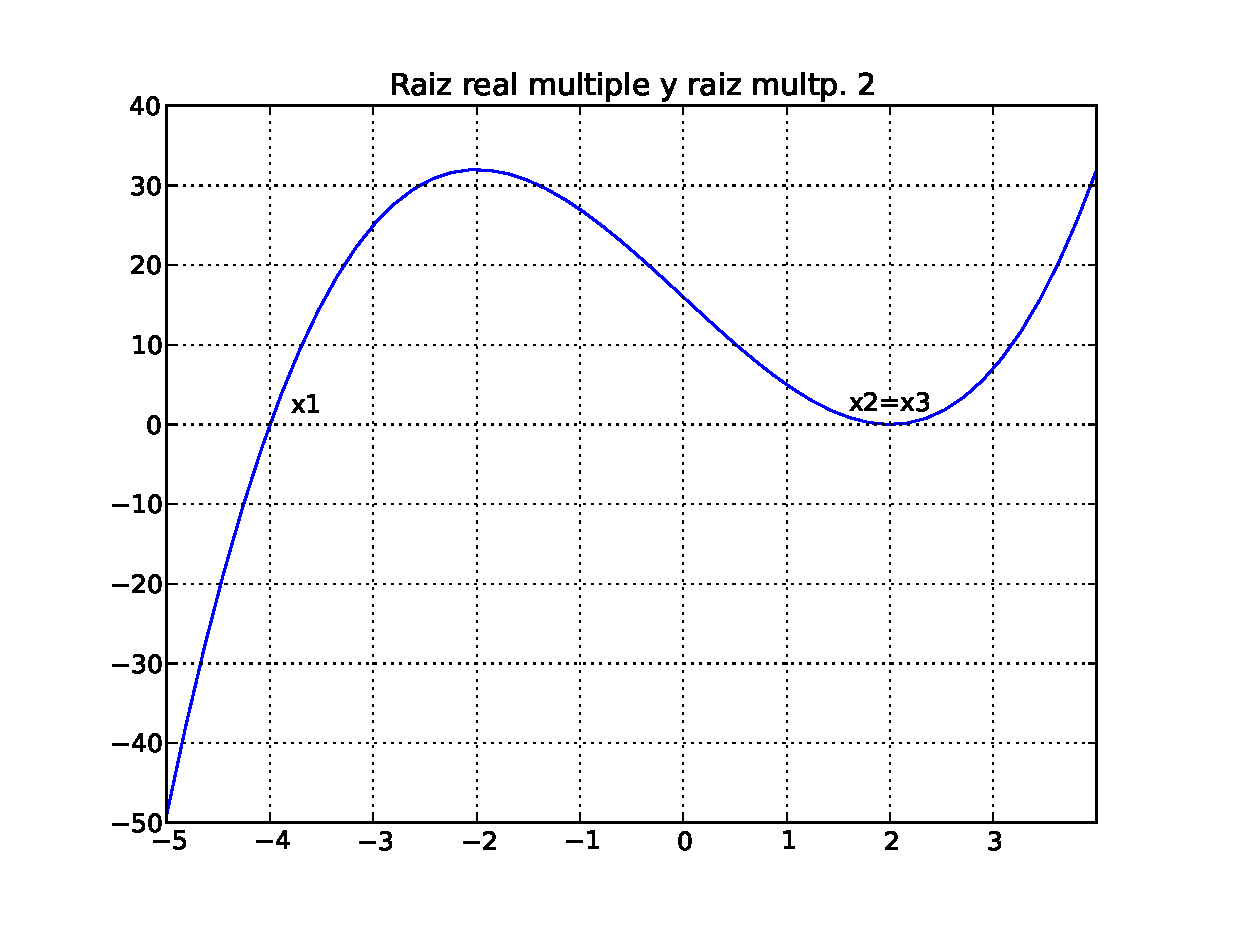
\includegraphics[scale=0.3]{Imagenes/raices03.eps} 
	\caption{Dos valores de las raíces coinciden.}
\end{figure}
\end{minipage}
\end{frame}
\begin{frame}[fragile]
\setbeamerfont{caption}{size=\scriptsize}
\captionsetup{justification=centering}
\frametitle{Raíz real y un par conjugado complejo}
\begin{minipage}{5cm}
\fontsize{12}{12}\selectfont
\begin{align*}
f(x) &= x^{3} - 2 \: x^{2} - 3 \: x + 10  \\
&= (x + 2)(x - (2 + i))* {}\\
&* (x - (2 - i))
\end{align*}
Las raíces son:
\begin{align*}
x_{1} &= -2 \\
x_{2} &= 2 + i \\
x_{3} &= 2 - i \\
\end{align*}
\end{minipage}
\hspace{0.5cm}
\begin{minipage}{4.5cm}
\begin{figure}
	\centering
	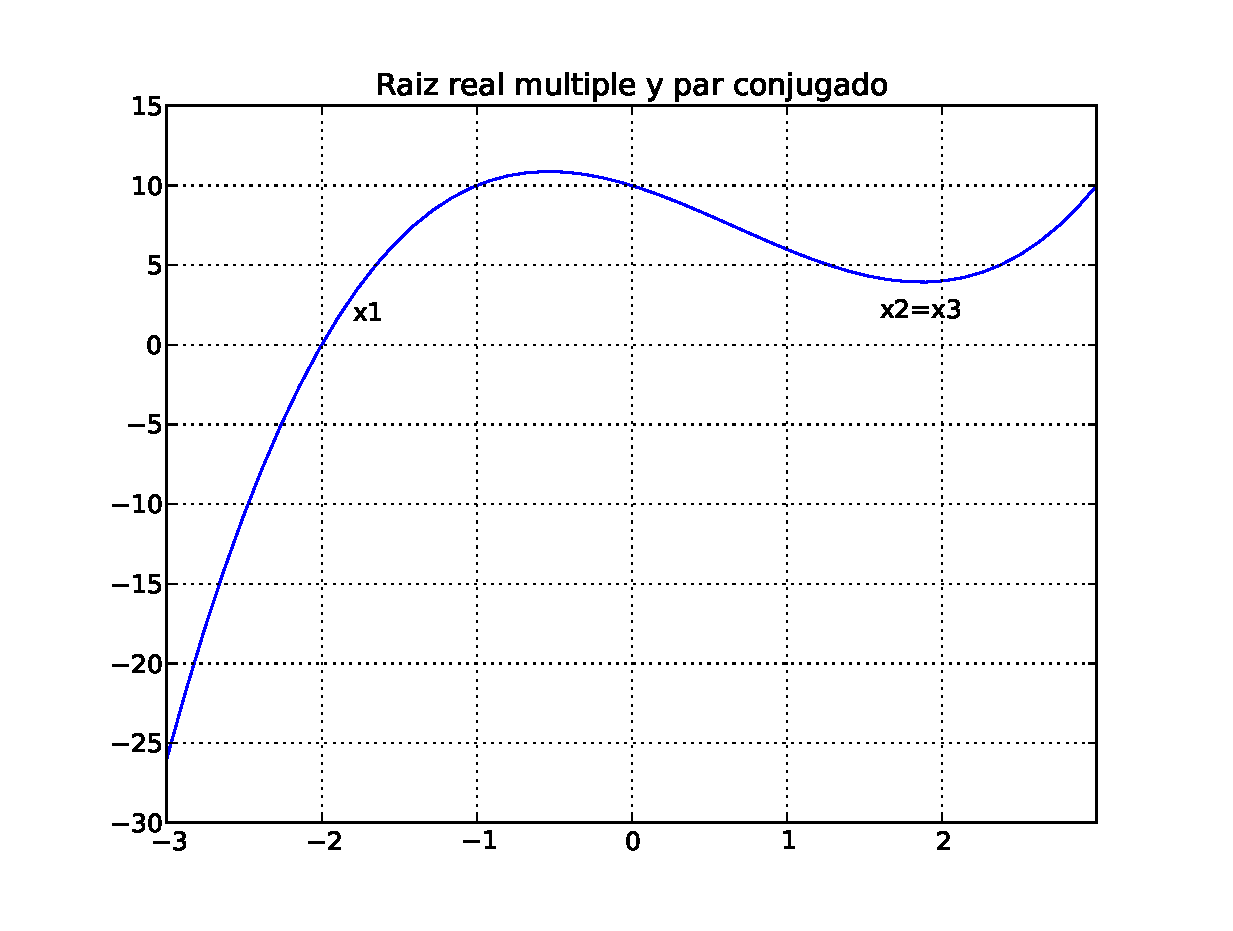
\includegraphics[scale=0.3]{Imagenes/raices04.eps} 
	\caption{Dos valores de las raíces son complejos.}
\end{figure}
\end{minipage}
\end{frame}
\section{Funciones algebraicas y trascendentales}
\frame{\tableofcontents[currentsection, hideothersubsections]}
\subsection{Funciones algebraicas}
\begin{frame}
\frametitle{Funciones algebraicas}
Sea $g = f(x)$ la función expresada como
\[ f_{n} \: y^{n} + f_{n-1} \: y^{n - 1} + \ldots + f_{1} \: y + f_{0} = 0 \]
Donde $f_{i}$ es un polinomio de orden $i$ en $x$.
\end{frame}
\begin{frame}
\frametitle{Funciones algebraicas}
Los polinomios son un caso simple de funciones algebraicas que se representan generalmente como
\[f_{n}(x) = a_{0} + a_{1} \: x + a_{2} \: x^{2}+ \ldots +a_{n} \: x^{n} \]
Donde $n$ es el orden del polinomio.
\end{frame}
\subsection{Funciones trascendentales}
\begin{frame}
\frametitle{Funciones trascedentales}
Son aquellas funciones que no son algebraicas.
\\
\bigskip
Comprenden a las funciones trigonométricas, exponenciales, logarítmicas, entre otras.
\\
\bigskip
\pause

Ejemplos:
\begin{align*}
f(x) &= ln(x^{2} - 1) \\
g(x) &= e^{-0.2 \: x} \sin(3 \: x - 5)
\end{align*}
\end{frame}
\subsection{Encontrar las raíces}
\begin{frame}
\frametitle{Encontrar las raíces}
Los métodos numéricos estándar para encontrar raíces pueden clasificarse en dos rubros:
\\
\bigskip
\azulfuerte{1.} La determinación de las raíces reales de ecuaciones algebraicas y trascendentales.
\\
\bigskip
\pause
Las técnicas a emplear en estos casos se diseñaron con el fin de encontrar el valor de una raíz simple de acuerdo con un conocimiento previo de su posición aproximada.
\end{frame}
\begin{frame}
\frametitle{Encontrar las raíces}
\azulfuerte{2.} La determinación de todas las raíces reales y complejas de un polinomio, para lo cual los métodos numéricos estén diseñados específicamente para polinomios. 
\\
\bigskip
\pause
Determinan sistemáticamente todas las raíces del polinomio en lugar de hacerlo sólo con una, dada la posición aproximada.
\end{frame}
\section{Método de incrementos sucesivos}
\frame{\tableofcontents[currentsection, hideothersubsections]}
\subsection{El método de incrementos sucesivos}
\begin{frame}
\frametitle{Método de incrementos sucesivos}
Podemos aproximar mucho mejor las raíces de una función, cuando la graficamos.
\\
\bigskip
Con una gráfica general de unos cuantos puntos, tendríamos lo necesario para considerar los valores de las raíces.
\end{frame}
\begin{frame}
\frametitle{Método de incrementos sucesivos}
El método de búsqueda incremental es una herramienta útil que podemos adoptar en conjunto con otras estrategias de cálculo de raíces.
\\
\bigskip
Éste método no nos ofrece más que una referencia sobre el intervalo en dónde podría(n) estar la(esas) raíces.
\end{frame}
\begin{frame}
\frametitle{Método de incrementos sucesivos}
La idea básica detrás del método de búsqueda incremental es simple: si $f(x_{1})$ y $f(x_{2})$ tienen signos opuestos, entonces hay al menos una raíz en el intervalo $(x_{1}, x_{2})$.
\end{frame}
\begin{frame}[fragile]
\frametitle{Caso en donde es posible encontrar la raíz}
\begin{figure}
	\centering
	\includestandalone{Figuras/figura_raices_01}
	\caption{Los puntos de la función evaluada en los extremos tienen signos contrarios.}
\end{figure}
\end{frame}
\begin{frame}[fragile]
\frametitle{Caso en donde no es posible encontrar la raíz}
\begin{figure}
	\centering
	\includestandalone{Figuras/figura_raices_02}
	\caption{Los puntos de la función evaluada en los extremos tienen el mismo signo.}
\end{figure}
\end{frame}
\begin{frame}
\frametitle{Cuando hay una raíz}
Si el intervalo es lo suficientemente pequeño, es probable que contenga una sola raíz.
\\
\bigskip
Así, los ceros de $f(x)$ puede ser detectados mediante la evaluación de la función en  intervalos $\Delta \: x$ y mirando cuando se presente un cambio de signo en la función.
\end{frame}
\begin{frame}
\frametitle{Consideraciones con el método}
Hay varios problemas con el método de incrementos sucesivos:
\setbeamercolor{item projected}{bg=purple!70!black,fg=white}
\setbeamertemplate{enumerate items}[circle]
\begin{enumerate}[<+->]
\item Es posible perder dos raíces muy próximas entre sí, si el incremento de búsqueda $\Delta \: x$ es mayor que la separación de las raíces.
\item Una raíz doble (dos raíces que coinciden) no será detectada.
\item Algunas singularidades de $f(x)$ se puede confundir con raíces. Por ejemplo, $f(x) = \tan x$. Tiene cambios de signo en $x = \pm 1/2 n\pi$ con $n = 1, 3, 5,\ldots$
\end{enumerate}
\end{frame}
\begin{frame}
\frametitle{Casos en donde no hay una raíz}
\begin{figure}
	\centering
	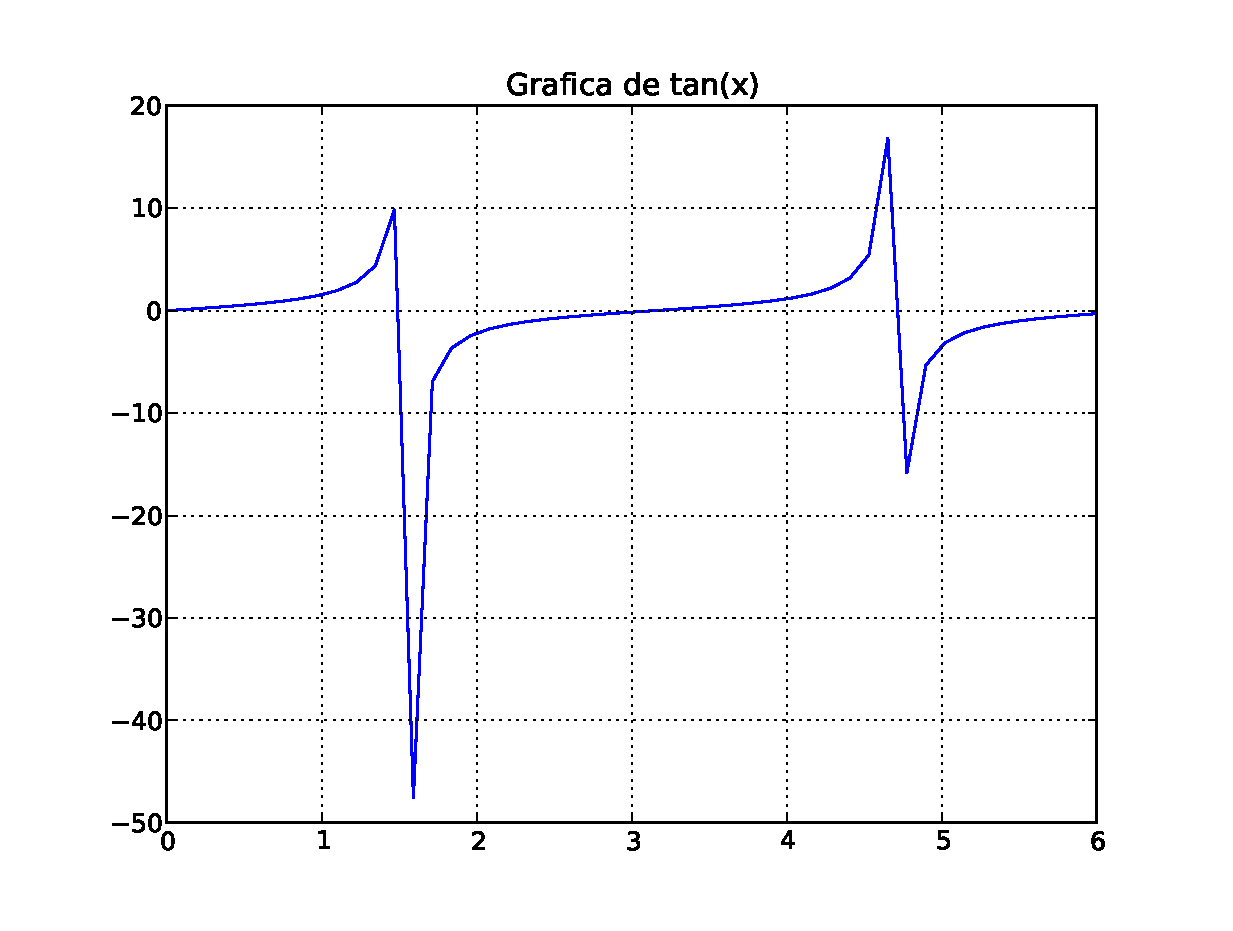
\includegraphics[scale=0.4]{Imagenes/raices05.eps}
	\caption{Estos puntos no son ceros verdaderos, ya que la función no cruza el eje $x$.}
\end{figure}
\end{frame}
\subsection{Código Método de incrementos sucesivos}
\begin{frame}
\frametitle{Código Método de incrementos sucesivos}
El código busca un cero de la función $f$ que proporciona el usuario en el intervalo
$(a, b)$ en incrementos de $dx$.
\\
\bigskip
Se devuelve el intervalo $(x_{1}, x_{2})$ donde se encuentra la raíz, si la búsqueda
se ha realizado correctamente; se devuelve $x_{1} = x_{2} = \mathsf{None}$ cuando no se encontraron raíces.
\end{frame}
\begin{frame}
\frametitle{Código Método de incrementos sucesivos}
Luego de que se encontró la primera raíz, (la más cercana al punto $a$), se puede llamar de nuevo al procedimiento, sustitiyendo $x_{2}$ con el fin de encontrar la siguiente raíz. 
\\
\bigskip
Esto se puede repetir siempre y cuando se detecta una raíz.
\end{frame}
\begin{frame}[fragile]
\frametitle{Función \azulfuerte{\texttt{buscaraiz}}}
\begin{lstlisting}[caption=Función buscaraiz, style= FormattedNumber, basicstyle=\linespread{1.1}\ttfamily=\small, columns=fullflexible]
def buscaraiz(f, a, b, dx):
    x_1_ = a; f_1_ = f(a)
    x_2_ = a + dx; f_2_ = f(x_2_)
    while f_1_ * f_2_ > 0.0:
        if x_1_ >= b: return None
        x_1_ = x_2_; f_1_ = f_2_
        x_2_ = x_1_ + dx; f_2_ = f(x_2_)
    else:
        return x_1_, x_2_
\end{lstlisting}
\end{frame}
\subsection{Ejercicio}
\begin{frame}
\frametitle{Ejemplo para encontrar una raíz}
Usa el método de incrementos sucesivos con espaciamientos de $\Delta x= 0.2$, para estimar la raíz con el valor positivo más pequeño de la función:
\[ f(x) = x^{3} - 10 x^{2} + 5\]
\end{frame}
\begin{frame}
\frametitle{¿Cómo resolver el problema?}
Como el ejercicio pide que se localice la raíz positiva más pequeña, habrá que tener una idea sobre el comportamiento de la función.
\\
\bigskip
Para ello, graficamos en un intervalo inicial, considera que hay potencias al cubo.
\end{frame}
\begin{frame}
\frametitle{Gráfica inicial de la función}
\begin{figure}
	\centering
	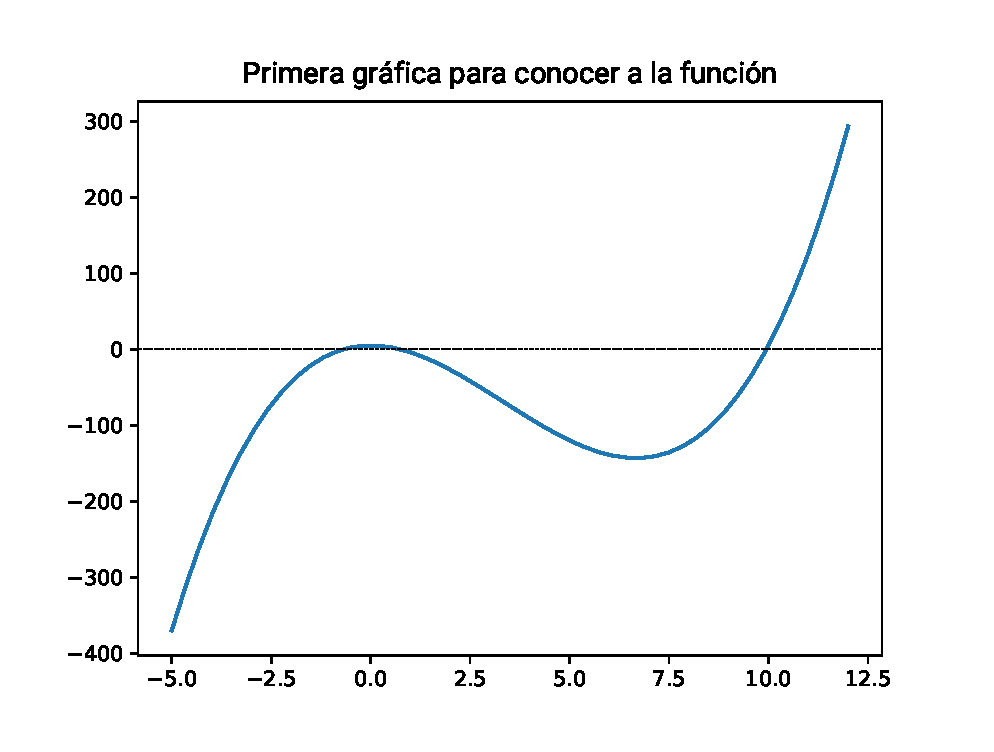
\includegraphics[scale=0.5]{Imagenes/aprox_sucesivas_01.eps}
	\caption{De la gráfica vemos que hay tres raíces, que cruzan el eje $y=0$.} 
\end{figure}
\end{frame}
\begin{frame}
\frametitle{Acotando el problema}
Como se nos pide el valor de la raíz positiva más pequeña, descartamos las raíz negativa y la otra raíz positiva.
\\
En la siguiente gráfica se reduce el intervalo sobre el eje $x$ para tener una mejor vista.
\end{frame}
\begin{frame}
\frametitle{El intervalo de la gráfica se ha acotado}
\begin{figure}
	\centering
	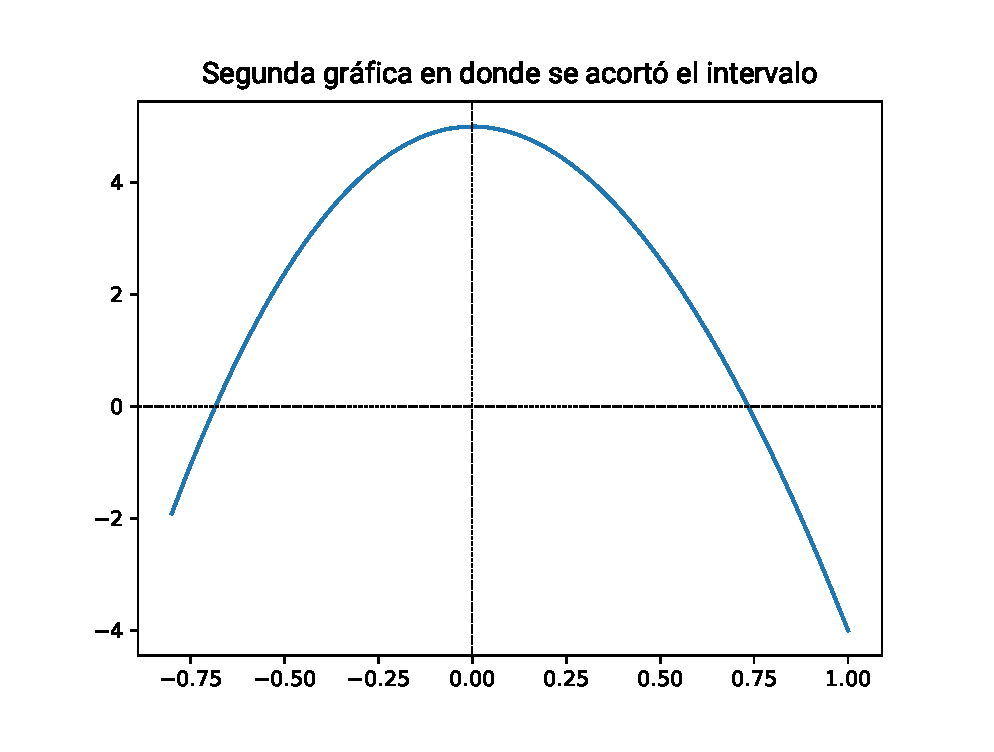
\includegraphics[scale=0.5]{Imagenes/aprox_sucesivas_02.eps}
	\caption{Se aprecia mucho mejor al reducir el intervalo, pero nos falta aún estimar con el código el intervalo donde está la raíz positiva más pequeña.} 
\end{figure}
\end{frame}
\begin{frame}[fragile]
\frametitle{Ahora con \python}
\begin{lstlisting}[caption=Solución con python, style=FormattedNumber, basicstyle=\linespread{1.1}\ttfamily=\small, columns=fullflexible]
def f(x): return x**3 - 10 * x**2 + 5.

a, b, dx = (0.0, 1.5, 0.2)

print ('El intervalo es: ')
x_1_, x_2_ = buscaraiz(f, a, b, dx)
print (x_1_, x_2_)
\end{lstlisting}
\end{frame}
\begin{frame}
\frametitle{El intervalo de trabajo}
\begin{figure}
	\centering
	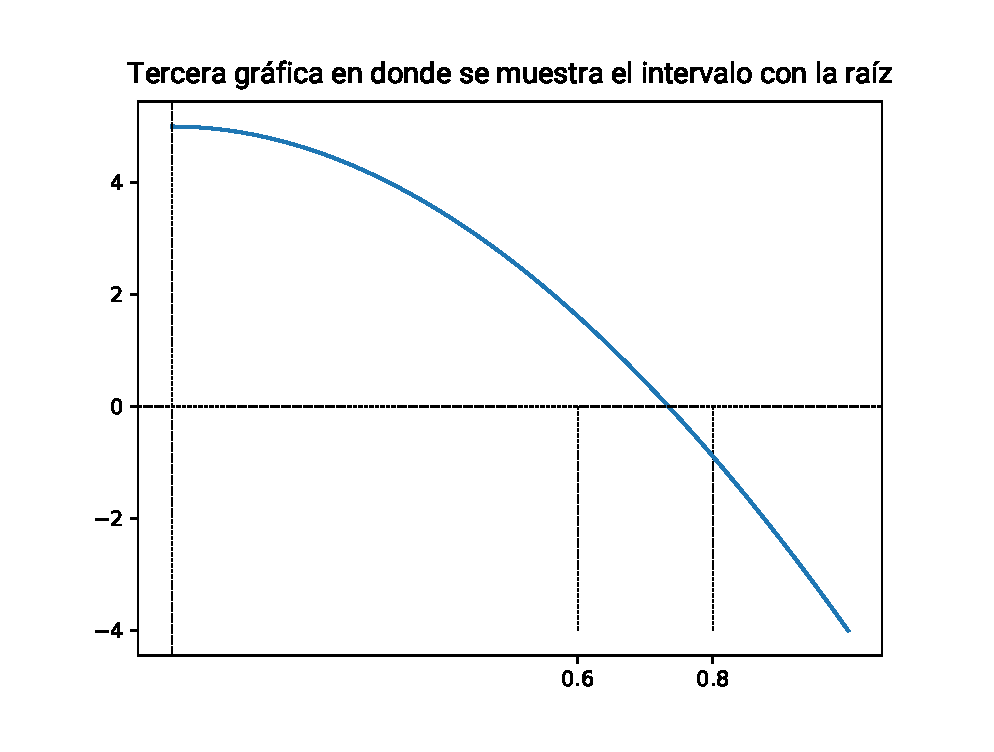
\includegraphics[scale=0.5]{Imagenes/aprox_sucesivas_03.eps}
	\caption{El código devuelve el intervalo de interés, por lo que ahora hay que usar alguna técnica para conocer el valor de la raíz.} 
\end{figure}
\end{frame}
\section{Métodos para el cálculo de raíces}
\frame{\tableofcontents[currentsection, hideothersubsections]}
\subsection{Método de Bisección}
\begin{frame}
\frametitle{Método de Bisección}
Después de que se ha identificado una raíz $f(x) = 0$ en el intervalo $(x_{1}, x_{2})$, disponemos de varios métodos para encontrar el valor de la raíz.
\end{frame}
\begin{frame}
\frametitle{Método de Bisección}
El método de bisección logra esta tarea: \textcolor{red}{el intervalo se reduce sucesivamente a la mitad  hasta que se vuelve suficientemente pequeño}. 
\end{frame}
\begin{frame}
\frametitle{Método de Bisección}
La técnica de bisección no es el método más rápido disponible, pero es el más fiable.
\\
\bigskip
Una vez que una raíz se ha encontrado en un intervalo, nos podemos acercar a ella.
\end{frame}
\begin{frame}
\frametitle{Funcionamiento del método}
El método de bisección utiliza el mismo principio que el de incrementos sucesivos: si hay una raíz en el intervalo $(x_{1}, x_{2})$, entonces revisa si $f(x_{1})*f(x_{2})<0$.
\end{frame}
\begin{frame}
\frametitle{Funcionamiento del método}
Con el fin de reducir a la mitad el intervalo, se calcula $f(x_{3})$, donde $x_{3} = (x1 + x2)/2$ es el punto medio del intervalo.
\end{frame}
\begin{frame}
\frametitle{Descripción gráfica del método de bisección}
\setbeamercovered{invisible}
\begin{figure}
	\centering
	\includestandalone{Figuras/biseccion_01}
\end{figure}
\end{frame}
\begin{frame}
\frametitle{Funcionamiento del método}
Si $f(x_{1})*f(x_{3}) < 0$, entonces la raíz debe estar en $(x_{1}, x_{3})$ entonces re-emplazamos del intervalo inicial $x_{2}$ por $x_{3}$, y se repite la división del intervalo.
\setbeamercovered{invisible}
\pause
\begin{figure}
	\centering
	\includestandalone{Figuras/biseccion_02}
\end{figure}
\end{frame}
\begin{frame}
\frametitle{Funcionamiento del método}
De lo contrario, la raíz se encuentra en el intervalo $(x_{3}, x_{2})$, en tal caso, se sustituye $x_{3}$ por $x_{1}$, y se repite la división del intervalo.
\end{frame}
\begin{frame}
\frametitle{¿Hasta cuando se repite la división del intervalo?}
En cualquiera de los casos, el nuevo intervalo $(x_{1}, x_{2})$ es la mitad del tamaño del intervalo original.
\\
\bigskip
La bisección es repite hasta que el intervalo se ha reducido a un valor $\varepsilon$ pequeño, de modo que
\[ \vert x_{2} - x_{1} \vert \leq \varepsilon\]
\end{frame}
\begin{frame}
\frametitle{Estimar el número de divisiones del intervalo}
Es fácil calcular el número de bisecciones necesarias para alcanzar el valor de $\varepsilon$.
\\
\bigskip
\pause
El intervalo inicial $\Delta \: x$, se reduce a $\Delta \: x /2$ en la primera bisección, $\Delta \: x /2^{2}$ en la segunda, luego de $n$ bisecciones, $\Delta \: x /2^{n}$.
\\
\bigskip
\pause
Haciendo $\Delta \: x /2^{n} = \varepsilon$, resolvemos para $n$
\[ n = \dfrac{ln(\vert \Delta x \vert/ \varepsilon)}{ln 2}\]
\end{frame}
\begin{frame}[allowframebreaks, fragile]
\frametitle{Función el método de bisección}
\begin{lstlisting}[caption=Método de bisección con \python, style=FormattedNumber, basicstyle=\linespread{1.1}\ttfamily=\small, columns=fullflexible]
def biseccion(f, x_1_, x_2_, switch = 1, tol = 1.0e-9):
    f_1_ = f(x_1_)
    if f_1_ == 0.0: return x_1_
    
    f_2_ = f(x_2_)
    if f_2_ == 0.0: return x_2_
    
    if sign(f_1_) == sign(f_2_):
        print('La raiz no esta en el intervalo')

    n = int(math.ceil(math.log(abs(x_2_ - x_1_)/tol)/math.log(2.0)))
    
    for i in range(n):
        x3 = 0.5 * (x_1_ + x_2_); f3 = f(x_3_)
        if (switch == 1) and (abs(f_3_) > abs(f_1_)) \
                    and (abs(f_3_) > abs(f_2_)):
                        
            return None
        
        if f_3_ == 0.0: return x_3_

        if sign(f_2_) != sign(f_3_): x_1_ = x_3_; f_1_ = f_3_
        else: x_2_ = x_3_; f_2_ = f_3_
    
    return (x_1_ + x_2_)/2.0
\end{lstlisting}
\end{frame}
\begin{frame}
\frametitle{El argumento \texttt{switch}}
Al establecer el valor del argumento \texttt{switch} $=1$, forzamos
la rutina para verificar si la magnitud de $f(x)$ disminuye con cada intervalo
a la mitad.
\end{frame}
\begin{frame}
\frametitle{El argumento \texttt{switch}}
Si no lo hace, algo puede estar mal: probablemente la \enquote{raíz}, no es una raíz
en absoluto, pero un polo.
\\
\bigskip
En ese caso, se devuelve \texttt{raíz = None}. Porque esta característica no siempre es
deseable, el valor predeterminado es \texttt{switch} $=0$.
\end{frame}
\begin{frame}[fragile]
\frametitle{¿Qué hace la función \azulfuerte{\texttt{ceil}}?}
La función \texttt{ceil} devuelve el menor entero mayor o igual a $x$.
\\
\medskip
Ejemplos:\\
\medskip
\verb|>>>ceil(1.1) # 2.0| \\
\verb|>>>ceil(1.6) # 2.0| \\
\verb|>>>ceil(-1.1) # -1.0| \\
\verb|>>>ceil(-1.6) # -1.0|
\end{frame}
\begin{frame}[fragile]
\frametitle{Ejemplo}
Calcular la raíz de 
\[ x^{3} - 10 \; x^{2} + 5 = 0 \]
que se encuentra en el intervalo $(0,1)$, con una precisión de 4 dígitos. 
\\
\bigskip
¿Cuántas evaluaciones se requieren para encontrar la raíz?
\end{frame}
\begin{frame}[fragile]
\frametitle{Ejemplo}
Como primer punto, generamos una gráfica para tener una idea del comportamiento de la función
\begin{figure}
	\centering
	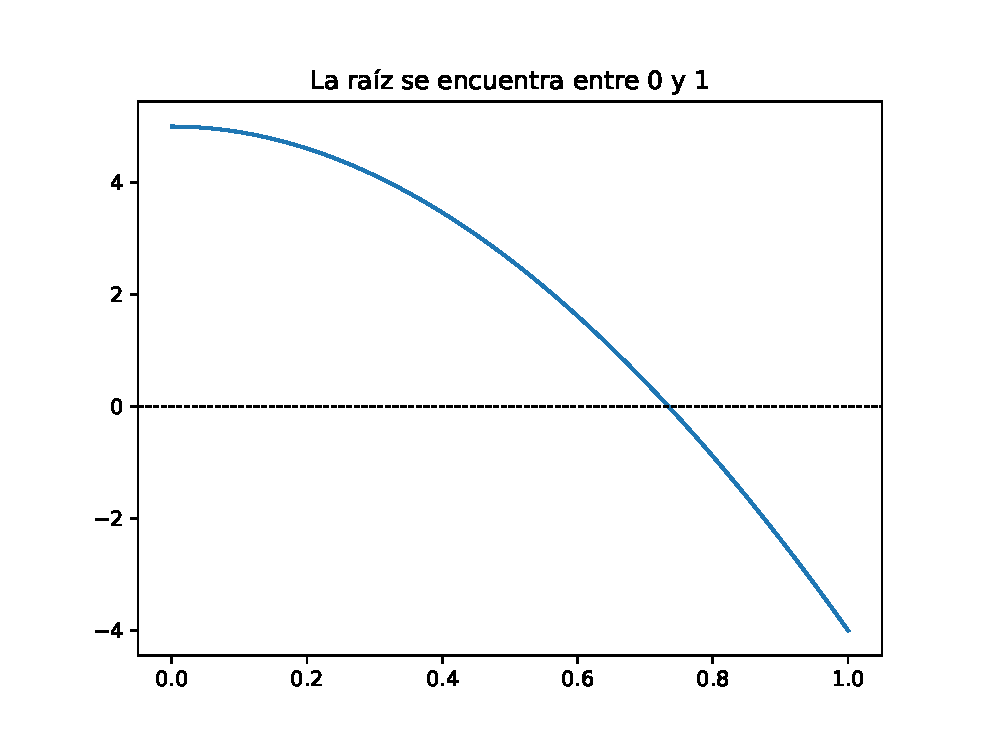
\includegraphics[scale=0.5]{Imagenes/Ejercicio_4_2_Libro.eps}
\end{figure}
\end{frame}
\begin{frame}[fragile]
\frametitle{Solución}
\begin{lstlisting}[caption=Solución al ejercicio, style=FormattedNumber, basicstyle=\linespread{1.1}\ttfamily=\small, columns=fullflexible]
from ModuloRaices import biseccion

def f(x): return x**3 - 10.0*x**2 + 5.0

raiz = biseccion(f, 0., 1.0, tol = 1.0e-4)

print('raiz=', '{:6.4f}'.format(raiz))
\end{lstlisting}
\end{frame}
\begin{frame}[fragile]
\frametitle{Solución gráfica}
Una vez calculada la raíz, podemos presentarla en la gráfica
\begin{figure}
	\centering
	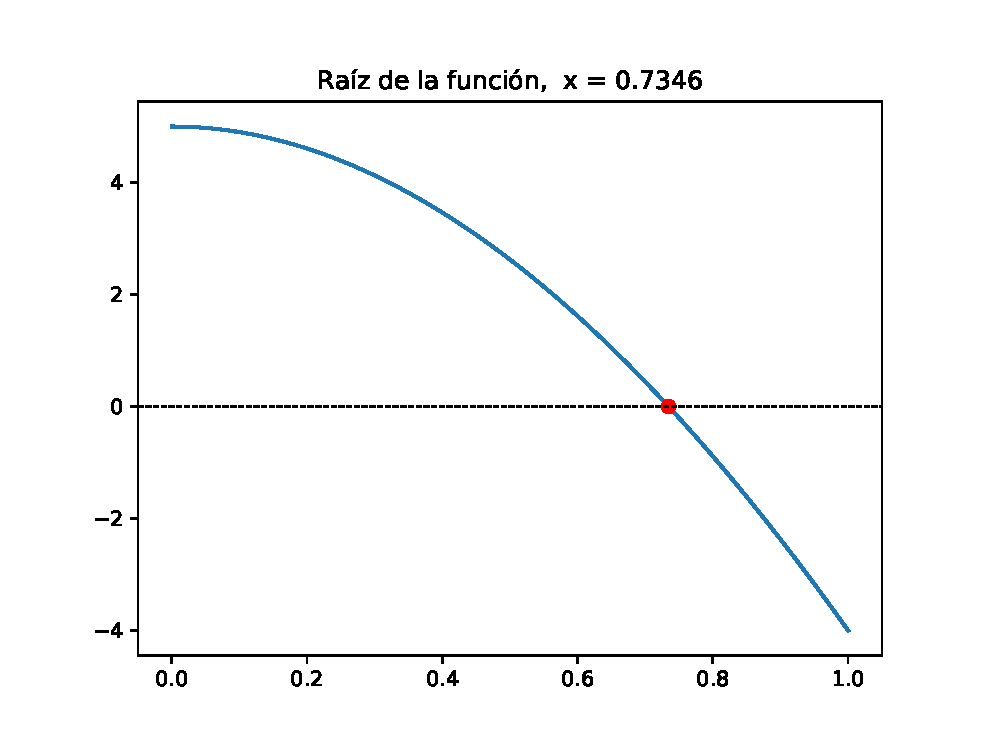
\includegraphics[scale=0.5]{Imagenes/Ejercicio_4_2_02_Libro.eps}
\end{figure}
\end{frame}
% \begin{frame}[fragile]
% \frametitle{Algoritmo para el método de bisección}
% 	\begin{lstlisting}
%     for i in np.arange(n):
%         x3 = 0.5*(x1 + x2); f3 = f(x3)
%         if (switch == 0) and (abs(f3) > abs(f1)) \
%                         and (abs(f3) > abs(f2)):
%             return None
%         if f3 == 0.0: return x3
%         if f2*f3 < 0.0:
%             x1 = x3; f1 = f3
%         else:
%             x2 =x3; f2 = f3
%     return (x1 + x2)/2.0
% 	\end{lstlisting}

% \end{frame}
% \begin{frame}
% Haciendo que la variable \texttt{switch} = 1, se forza la rutina para comprobar si la magnitud de $f(x)$ disminuye con la reducción a la mitad de cada intervalo.
% \end{frame}
% \begin{frame}
% Si no es así, algo anda mal (probablemente la \enquote{raíz} no es una raíz en absoluto, sino una singularidad) y se devuelve la \texttt{raíz} = \texttt{None}.
% \\
% \bigskip
% Dado que esta característica no siempre es deseable, el valor predeterminado es \texttt{switch}=0.
% \end{frame}
% \begin{frame}
% Veamos lo que hace la variable \texttt{switch}:
% \\
% \medskip
% Hasta el momento no nos hemos fijado en la magnitud de $f(x_{1})$ y $f(x_{2})$, sólo y en el signo del respectivo producto, pero ahora, tomamos en cuenta la magnitud tanto de los puntos evaluados en la función como del producto mismo.
% \\
% \medskip
% Consideremos le primer caso de la función $f(x)$, donde ya sabemos que hay una raíz en el intervalo $[0.6,0.8]$
% \end{frame}
% \begin{frame}[fragile]
% \frametitle{El valor por defecto de \texttt{switch} = 0}
% \begin{tabular}{l | l | l | l | c}
% $x_{1}$ & $x_{2}$ & $f(x_{1})$ & $f(x_{2})$ & $f(x_{1})f(x_{2})$ \\ \hline
% 0.0 & 0.2 & 5.0 & 4.608 & 23.04 \\ \hline
% 0.2 & 0.4 & 4.608 & 3.464 & 15.9621 \\ \hline
% 0.4 & 0.6 & 3.464 & 1.616 & 5.5978 \\ \hline
% 0.6 & 0.8 & 1.616 & -0.888 & -1.4350 \\ \hline
% 0.8 & 1.0 & -0.888 & -4.0 & 3.552 \\ \hline
% 1.0 & 1.2 & -4.0 & -7.672 & 30.688
% \end{tabular}
% %\begin{tikzpicture}[overlay]
% % Define the circle paths
% %	\draw [blue](1.north west) -- (1.north east) -- (2.south east) -- (2.south west) -- cycle;
% %	\draw [red](3.north west) -- (3.north east) -- (4.south east) -- (4.south west) -- cycle;
% %\end{tikzpicture}
% \end{frame}
% \begin{frame}[fragile]
% Del código tenemos que:
% \begin{verbatim}
% if (switch == 0) and (abs(f3) > abs(f1)) \ 
%                  and (abs(f3) > abs(f2)):
%     return None
% \end{verbatim}
% \begin{tabular}{l  l | l | l}
% $abs(f3) > abs(f1)$ & $abs(f3) > abs(f2)$ & Expresión \\ \hline
% \texttt{True} & \texttt{True} & True \\ \hline

% \end{tabular}
% Aquí tendrán que completar la tabla de tal manera que revisen el resultado de la expresión compuesta.
% \end{frame}
% \begin{frame}
% \frametitle{Ejercicios}
% Implementa el método de bisección para calcular el(los) intervalo(s) y la(s) raíz(ces) de:
% \begin{eqnarray*}
% 	f(x) &=& x^{3} - 10x^{2} + 5 \\
% 	g(x) &=& x- \tan(x) \hspace{1cm} 0 \leq x \leq 20
% \end{eqnarray*}
% Con una tolerancia de $1\times 10^{-9}$
% \end{frame}
% \begin{frame}
% Toma en cuenta que $\tan(x)$ es singular y cambia de signo en $x = \pi/2, 3\pi/2,\ldots$. Para no confundir estos puntos para las raíces, hacemos \texttt{switch}= 1.
% \\
% \medskip
% La proximidad de las raíces a las singularidades es otro problema potencial que puede ser prevenido mediante el uso de $\Delta x$ pequeña, usa $x = 0.01$.
% \end{frame}
% \begin{frame}
% \frametitle{Graficas de las funciones y sus raíces}
% \begin{figure}
% 	\centering
% 	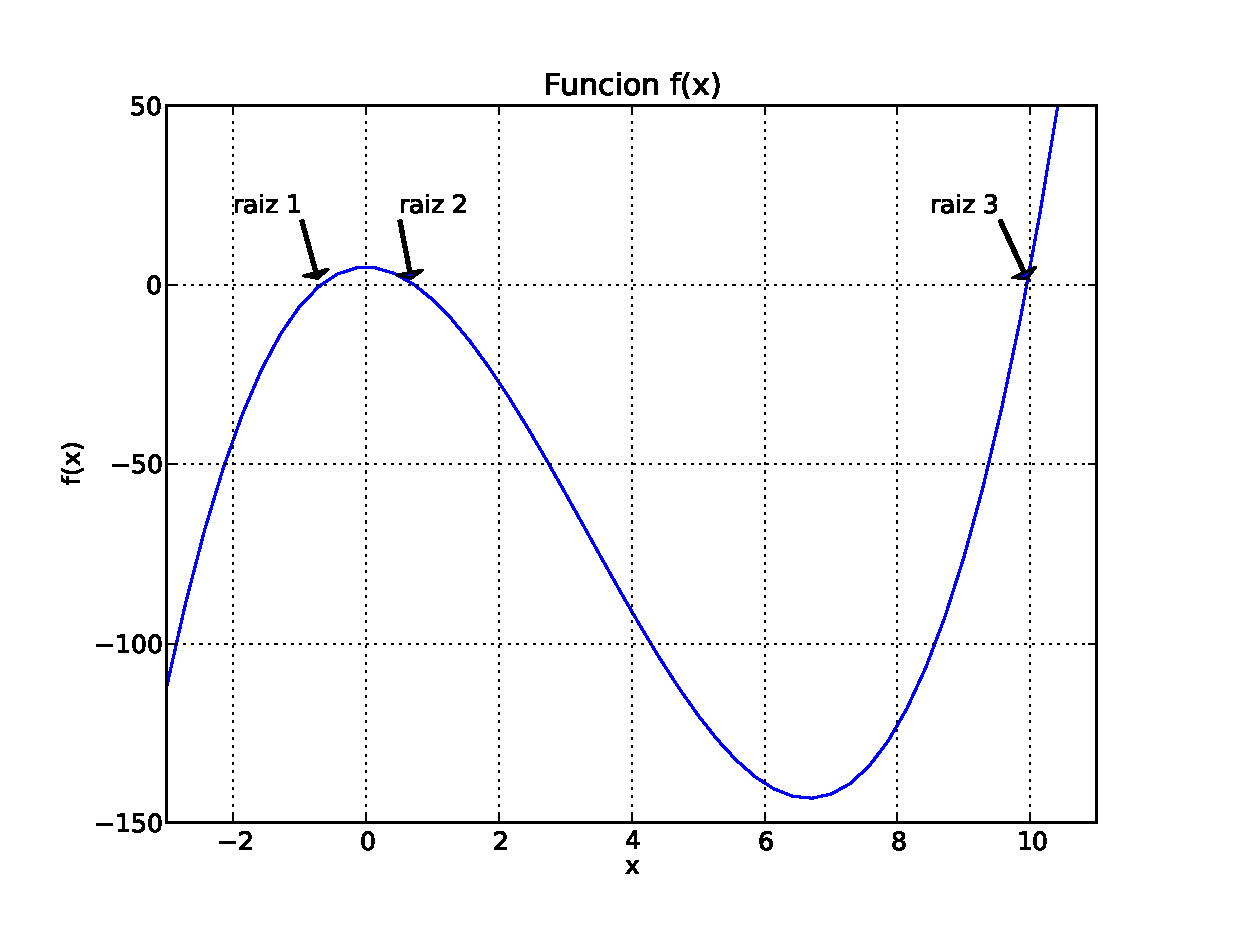
\includegraphics[scale=0.4]{ejercicio1_Biseccion.eps}<1>
% 	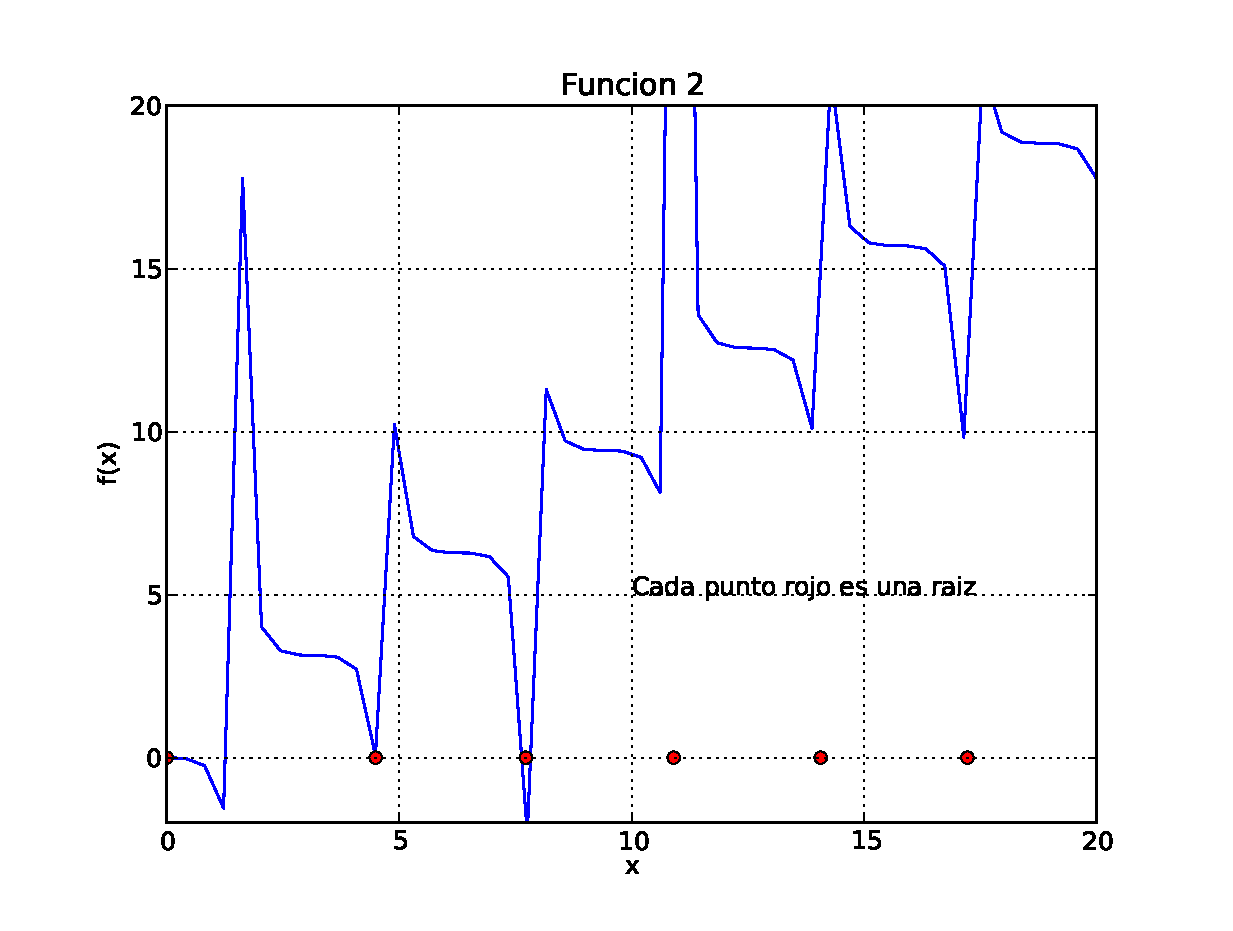
\includegraphics[scale=0.4]{ejercicio2_Biseccion.eps}<2>
% \end{figure}
% \end{frame}
% \begin{frame}
% \frametitle{Estrategia de solución}
% Para integrar los elementos que hemos visto:
% \begin{enumerate}
% \item Recuperamos el algoritmo que nos identifica en qué intervalo se encuentra una raíz.
% \item Aplicamos el algoritmo del método de bisección.
% \item Usamos un ciclo que nos revise en el dominio que se nos proporciona, si existe más de una raíz.
% \end{enumerate}
% \end{frame}
% \begin{frame}[fragile]
% \begin{lstlisting}
% def f(x): return x**3-10*x**2+5

% a,b,dx = (-2.0,11.0,0.02)
	
% print 'Intervalo (x1,x2)   raiz'
% while 1:
%     try:
%         x1, x2 = buscaraiz(f,a,b,dx)
%     except Exception, e:
%         print e; break
%     if x1 != None:
%         a = x2
%         root = bisect(f,x1,x2,0)
%         if raiz != None: print '(%2.4f, %2.4f) %2.8f' %(x1, x2, raiz)
% \end{lstlisting}
% \end{frame}
% \begin{frame}[fragile]
% \begin{lstlisting}
%     else:
%         print '\nHecho'
%         break
% \end{lstlisting}
% \end{frame}
\subsection{Método de Newton-Raphson}
\begin{frame}
\frametitle{Método de Newton-Raphson}
El método de Newton-Raphson es el algoritmo más conocido para encontrar raíces por una buena razón: es simple y rápido.
\end{frame}
\begin{frame}
\frametitle{Método de Newton-Raphson}
El único detalle es que utiliza la derivada $f^{\prime}(x)$ así como la función $f(x)$.
\\
\bigskip
Por tanto, en los problemas a resolver con este algoritmo, deberá de contemplarse que la derivada sea fácil de calcularse.
\end{frame}
\begin{frame}
\frametitle{Método de Newton-Raphson}
El método de N-R se obtiene de la expansión en series de Taylor de $f(x)$ alrededor de $x$:
\[ f(x_{i + 1})  = f(x_{i}) + f^{\prime}(x_{i})(x_{i + 1} - x_{i}) + O(x_{i + 1} - x_{i})^{2}\]
\end{frame}
\begin{frame}
\frametitle{Definición del método N-R.}
Si $x_{i + 1}$ es una raíz de $f(x)=0$, tenemos que:
\[ 0 = f(x_{i}) + f^{\prime}(x_{i})(x_{i + 1} - x_{i}) + O(x_{i + 1} - x_{i})^{2} \]
Suponiendo que $x_{i}$ está cerca de $x_{i + 1}$, podemos eliminar el último término de la ecuación y resolver para $x_{i+1}$, por lo que la fórmula de Newton-Raphson es:
\[ x_{i+1} = x_{i} - \dfrac{f(x_{i})}{f^{\prime}(x_{i})} \]
\end{frame}
\begin{frame}
\frametitle{Definición del método N-R.}
Si $x$ representa el valor verdadero de la raíz, el error en $x_{i}$ es $E_{i} =x - x_{i}$. 
\\
\bigskip
Se puede demostrar que si $x_{i + 1}$ se calcula de la expresión de N-R, el error es:
\[ E_{i + 1} = - \dfrac{f^{\prime \prime}(x_{i})}{2 \: f^{\prime}(x_{i})} \; E_{i}^{2}\]
Lo que nos dice que el método de N-R converge de manera cuadrática, es decir, el error es el cuadrado del error del punto previo.
\end{frame}
\begin{frame}[fragile]
\frametitle{Representación gráfica}
Podemos interpretar que $x_{i+1}$ es el punto en donde la tangente de $f(x_{i})$ cruza el eje de las $x$:
\begin{figure}
	\centering
	\includestandalone{Figuras/newton-raphson_01}
\end{figure}
\end{frame}
\begin{frame}[fragile]
\frametitle{Uso del método}
El método de N-R es sencillo: se aplica la expresión para $x_{i + 1}$ iniciando con un valor $x_{0}$, hasta alcanzar un criterio de convergencia:
\[ \vert x_{i+1} - x_{i} \vert < \varepsilon \]
\end{frame}
\begin{frame}[fragile]
\frametitle{Uso del método}
El algoritmo es el siguiente:
\setbeamercolor{item projected}{bg=purple!70!black,fg=white}
\setbeamertemplate{enumerate items}[circle]
\begin{enumerate}[<+->]
\item Sea $x$ un valor inicial para la raíz de $f(x)=0$.
\item Calcular $\Delta x = - f(x)/f^{\prime}(x)$.
\item Asignar $x \leftarrow x + \Delta x$ y se repiten los pasos 2-3, hasta alcanzar $\vert \Delta x \vert < \varepsilon$.
\end{enumerate}
\end{frame}
\begin{frame}[fragile]
\frametitle{Precaución con el método N-R}
Aunque el método de Newton-Raphson converge rápidamente cerca de la raíz, sus características globales de convergencia son pobres. 
\\
\bigskip
La razón es que la línea tangente no es siempre una aproximación aceptable de la función.
\end{frame}
\begin{frame}[fragile]
\frametitle{Precaución con el método N-R}
\begin{figure}
	\centering
	\includestandalone{Figuras/newton-raphson_02}
\end{figure}
\end{frame}
\begin{frame}[fragile]
\frametitle{Precaución con el método N-R}
\begin{figure}
	\centering
	\includestandalone{Figuras/newton-raphson_03}
\end{figure}
\end{frame}
% \subsection{Algoritmo para el método Newton-Raphson}
\begin{frame}
\frametitle{Algoritmo para el método Newton-Raphson}
La siguiente algoritmo para el método de Newton-Raphson supone que la raíz a calcularse inicialmente está en el intervalo $(a, b)$.
\end{frame}
\begin{frame}
\frametitle{Algoritmo para el método Newton-Raphson}
El punto medio del intervalo se utiliza como aproximación inicial de la raíz. Los extremos del intervalo se actualizan luego de cada iteración.
\\
\bigskip
Si una iteración del método Newton-Raphson no se mantiene dentro del intervalo, se descarta y se reemplaza con el método de bisección.
\end{frame}
\begin{frame}
\frametitle{Algoritmo para el método Newton-Raphson}
Ya que el método \funcionazul{newtonRaphson} utiliza la función $f(x)$, así como su derivada, (denotadas por $f$ y $df$) deben ser proporcionadas por el usuario.
\end{frame}
\begin{frame}[plain, allowframebreaks, fragile]
\frametitle{Algoritmo de \texttt{Newton-Raphson}}
\begin{lstlisting}[caption=Código del método N-R, style=FormattedNumber, basicstyle=\linespread{1.1}\ttfamily=\footnotesize, columns=fullflexible]
def newtonRaphson(f, df, a, b, tol = 1.0e-9):
    fa = f(a)
    if fa == 0.0: return a
    
    fb = f(b)
    if f(b) == 0.0: return b
    
    if fa * fb > 0.0: print ('La raiz no esta en el intervalo')
    
    x = 0.5 * (a + b)

    for i in range(30):
        fx = f(x)
        if abs(fx) < tol: return x

        if fa * fx < 0.0:
            b = x
        else:
            a = x; fa = fx

        dfx = df(x)
        
        try: dx = -fx/dfx
        except ZeroDivisionError: dx = b - a
        
        x =  x + dx
        
        if(b - x)*(x - a) < 0.0:
            dx = 0.5 * (b - a)
            x = a + dx
        
        if abs(dx) < tol*max(abs(b), 1.0): return x
    
    print('Son demasiadas iteraciones')
\end{lstlisting}
\end{frame}
\begin{frame}
\frametitle{Primer ejercicio}
Usando el método de Newton-Raphson, calcular las dos raíces de la función
\[ \sin \: x + 3 \: \cos \: x - 2 = 0  \]
en el intervalo $(-2, 2)$
\end{frame}
\begin{frame}
\frametitle{Primer paso: graficar la función}
La gráfica de la función en el intervalo dado es la siguiente:
\begin{figure}
	\centering
	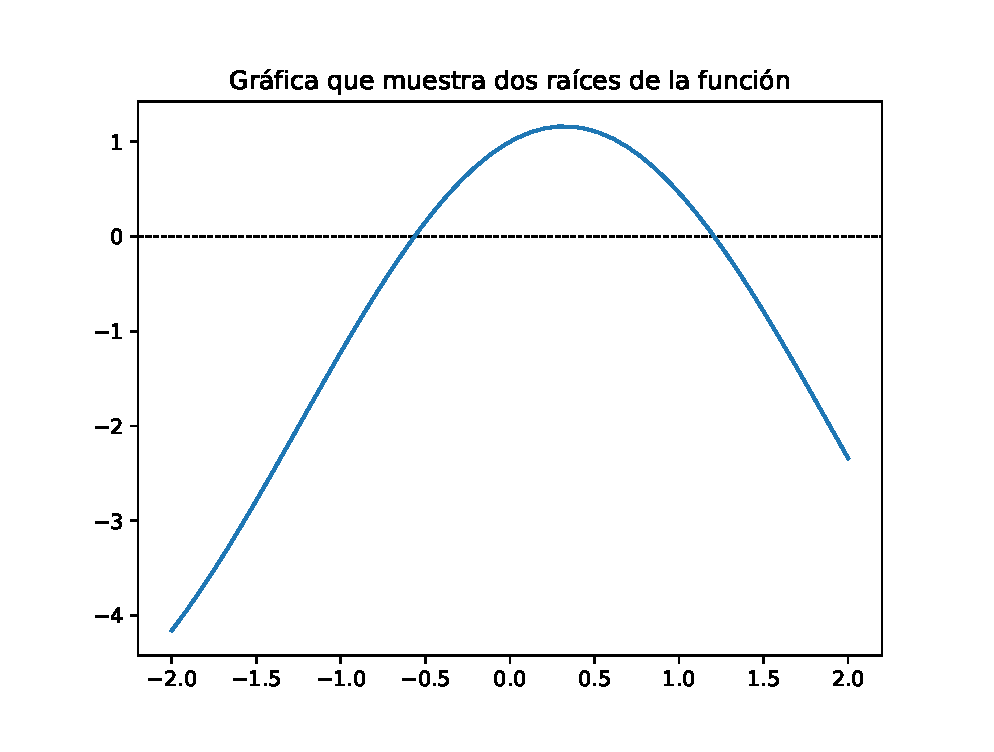
\includegraphics[scale=0.5]{Imagenes/Ejercicio_NR_Seno_01.eps}
\end{figure}
\end{frame}
\begin{frame}[fragile]
\frametitle{Intervalos de las raíces}
Con el método de incrementos sucesivos, estimamos cada intervalo donde se encuentran las raíces de la función.
\end{frame}
\begin{frame}[plain, fragile]
\frametitle{Intervalos de las raíces}
\begin{lstlisting}[caption=Intervalos para las raíces, style=FormattedNumber, basicstyle=\linespread{1.1}\ttfamily=\small, columns=fullflexible]
inicio, final, dx = -2., 2. , 0.01

a_1_, b_1_ = buscaraiz(f, inicio, final, 0.1)
print('Una raiz esta en  el intervalo [', a_1_, ',', b_1_ , ']')

inicio = b_1_

a_2_, b_2_ = buscaraiz(f, inicio, final, 0.1)
print('Una raiz esta en  el intervalo [', a_2_, ',', b_2_, ']')
\end{lstlisting}
\end{frame}
\begin{frame}[fragile]
\frametitle{Los intervalos}
El resultado que nos devuelve la función de incrementos sucesivos es:
\begin{verbatim}
Una raíz está en [ -0.6 , -0.5 ]
Una raíz está en [ 1.2 , 1.3 ]
\end{verbatim}
\end{frame}
\begin{frame}[allowframebreaks, plain, fragile]
\frametitle{Código completo}
\begin{lstlisting}[caption=Intervalos para las raíces, style=FormattedNumber, basicstyle=\linespread{1.1}\ttfamily=\small, columns=fullflexible]
from ModuloRaices import buscaraiz, newtonRaphson
import matplotlib.pyplot as plt
import numpy as np


def f(x): return np.sin(x) + 3 * np.cos(x) - 2
def df(x): return np.cos(x) - 3 * np.sin(x)


intervalo_1_ = []
intervalo_2_ = []

inicio, final, dx = -2., 2. , 0.01


a_1_, b_1_ = buscaraiz(f, inicio, final, 0.1)
print('Una raiz esta en [', round(a_1_, 2), ',', round(b_1_, 2) , ']')
intervalo_1_.append(a_1_)
intervalo_1_.append(b_1_)

inicio = b_1_
a_2_, b_2_ = buscaraiz(f, inicio, final, 0.1)
print('Una raiz esta en [', round(a_2_,2), ',', round(b_2_,2), ']')
intervalo_2_.append(a_2_)
intervalo_2_.append(b_2_)

raiz_1_ = newtonRaphson(f, df, intervalo_1_[0], intervalo_1_[-1], 1.e-4)
print(raiz_1_)

raiz_2_ = newtonRaphson(f, df, intervalo_2_[0], intervalo_2_[-1], 1.e-4)
print(raiz_2_)

x = np.linspace(-2, 2)
plt.axhline(y=0, ls='dashed', lw=0.7, color='k')
plt.plot(x, f(x), color='g')
plt.plot(raiz_1_, 0, 'ro', label='Raiz _1_ = ' + str(round(raiz_1_, 3)))
plt.plot(raiz_2_, 0, 'bo', label='Raiz _2_ = ' + str(round(raiz_2_, 3)))
plt.legend(loc='lower right')
plt.title('Grafica que muestra dos raices de la funcion')
plt.show()
\end{lstlisting}    
\end{frame}
\begin{frame}
\frametitle{Solución}
La gráfica de la función en el intervalo dado es la siguiente:
\begin{figure}
	\centering
	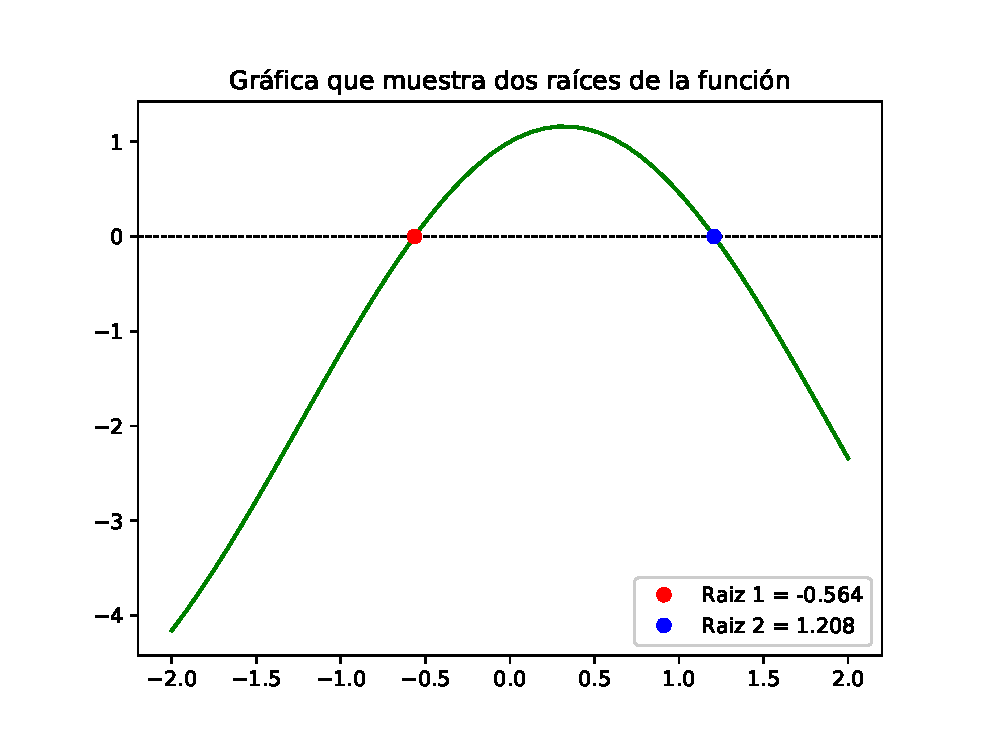
\includegraphics[scale=0.4]{Imagenes/Ejercicio_NR_Seno_02.eps}
	\caption{Implementando varias etapas, se calcularon las raíces de la función en el  intervalo.}
\end{figure}
\end{frame}
\begin{frame}
\frametitle{Ejercicio}
Encontrar la raíz positiva más pequeña de
\[ f(x) = x^{4} - 6.4 \: x^{3} + 6.45 \: x^{2} + 20.538 \: x - 31.752\]
Como en los ejercicios anteriores, es buena idea generar una gráfica de la función.
\end{frame}
\begin{frame}
\frametitle{Gráfica del ejercicio}
\begin{figure}
	\centering
	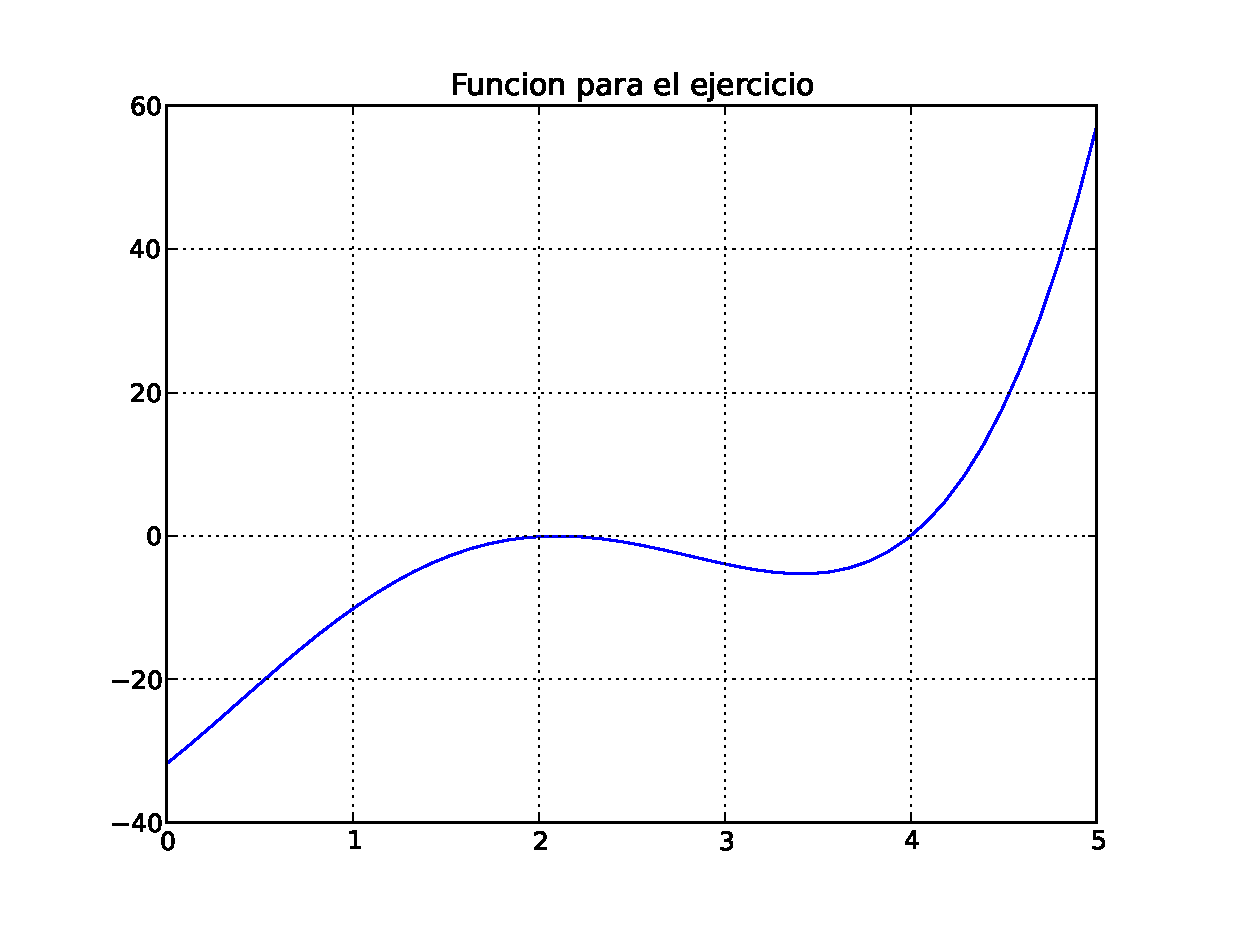
\includegraphics[scale=0.5]{Imagenes/raices08.eps}
\end{figure}
\end{frame}
\begin{frame}
\frametitle{Caso particular para esta función}
Al realizar un poco de álgebra, nos encontramos con lo siguiente:
\[ 0.002 (x - 4.) (5. x + 9.) (10. x - 21.)^{2} \]
La función tiene dos raíces reales y una de multiplicidad $2$.
\end{frame}
\begin{frame}
\frametitle{Ajuste al código de NR}
Como el método de NR se basa en detectar el cambio de signo en la función, en este caso, para una raíz con multiplicidad $2$, haremos un ajuste al código del método.
\end{frame} 	
% \begin{frame}[allowframebreaks,plain, fragile]
% \frametitle{Ejercicio}
% \begin{lstlisting}[caption=Código para el ejercicio, style=FormattedNumber, basicstyle=\linespread{1.1}\ttfamily=\small, columns=fullflexible]
% def f(x): return x**4 - 6.4 * x**3 + 6.45 * x**2 + 20.538 * x - 31.752
% def df(x): return 4.0 * x**3 - 19.2 * x**2 + 12.9 * x + 20.538

% def newtonRaphson(x, tol=1e-09):
%     for i in range(30):
%         dx = -f(x)/df(x)
%         x = x + dx
%         if abs(dx) < tol: return x,i
%     print('Son demasiadas iteraciones\n')

% raiz, numIter = newtonRaphson(2.0)

% print 'Raiz =',raiz
% print 'Numero de iteraciones =',numIter
% \end{lstlisting}
% \end{frame}
\begin{frame}
\frametitle{Solución del ejercicio}
\begin{figure}
	\centering
	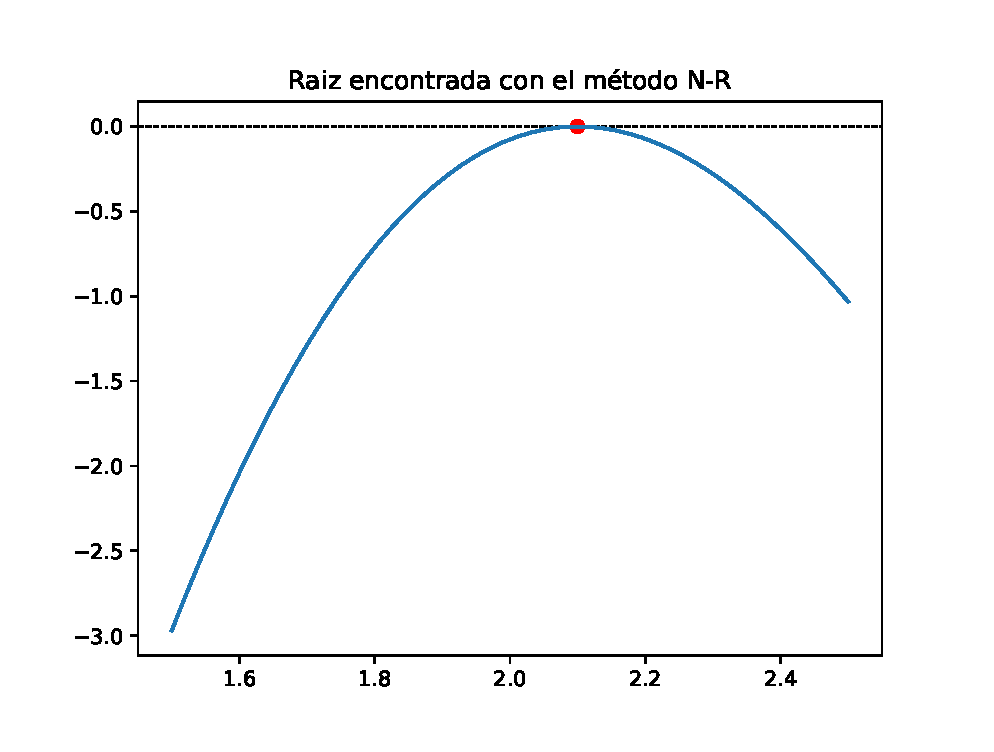
\includegraphics[scale=0.5]{Imagenes/Raiz_NR_02.eps}
\end{figure}
\end{frame}
\begin{frame}
\frametitle{Convergencia del método}
Se puede demostrar que la convergencia del método NR cerca de una raíz con multiplicidad es linear, más que cuadrática.
\\
\bigskip
\pause
La convergencia de una raíz múltiple se puede acelerar al cambiar la fórmula de NR.
\end{frame}
\begin{frame}
\frametitle{Ajuste a la función NR}
Se ajusta de la forma
\[ x_{i + 1} = x_{i} - m \; \dfrac{f(x_{i})}{f^{\prime}(x_{i})} \]
donde $m$ es la multiplicidad de la raíz (en el ejemplo, $m = 2$). Después de hacer los ajustes, el resultado se obtiene en $5$ iteraciones.
\end{frame}
%\begin{frame}
% \frametitle{Ejercicios}
% \begin{enumerate}
% \item Encuentra las raíces de $x \sin x + 3 \cos x - x = 0$ en el intervalo $(-6,6)$ \\
% \item Calcula todas las raíces reales de $x^{4} + 0.9x^{3} - 2.3x^{2} + 3.6x - 25.2 = 0$. \\
% \item Calcula todas las raíces reales de $x^{4} + 2x^{3} - 7x^{2} + 3 = 0$. \\
% \item Calcula todas las raíces de $\sin x - 0.1x = 0$.
% \end{enumerate}
% \end{frame}
\subsection{Método de la falsa posición}
\begin{frame}
\frametitle{Método de la falsa posición}
Este método es parecido al de bisección, ya que el intervalo que contiene a la raíz se va reduciendo.
\\
\bigskip
En vez de bisectar de manera monótona el intervalo, se utiliza una interpolación lineal ajustada a dos puntos extremos para encontrar la aproximación de la raíz.
\end{frame}
\begin{frame}
\frametitle{Método de la falsa posición}
La función está bien aproximada por la interpolación lineal, con lo que las raíces tendrán una buena precisión; la iteración convergerá más rápido que como ocurre con el método de bisección.
\end{frame}
\begin{frame}
\frametitle{Método de la falsa posición}	
Dado un intervalo $[a,c]$ que contenga a la raíz, la función lineal que pasa por $(a,f(a))$ y $(c,f(c))$ se escribe como:
\[ y = f(a) + \dfrac{f(c) - f(a)}{c - a} \: (x - a) \]
de donde se despeja $x$:
\[ x = a + \dfrac{c - a}{f(c) - f(a)} \: \big[ y - f(a)\big] \]
\end{frame}
\begin{frame}
\frametitle{Método de la falsa posición}
La coordenada $x$ en donde la línea intersecta al eje $x$ se determina al hacer $y=0$ en la ecuación anterior, por tanto:
\[ b = a - \dfrac{c - a}{f(c) - f(a)} \: f(a) = \dfrac{a \: f(c) - c \: f(a)}{f(c)-f(a)} \]
Después de encontrar $b$, el intervalo $[a, c]$ se divide en $[a, b]$ y $[b, c]$.
\end{frame}
\begin{frame}
\frametitle{Método de la falsa posición}
Si $f(a) \: f(b) \leq 0$, la raíz se encuentra en $[a, b]$; en caso contrario, está en $[b, c]$. 
\\
\bigskip
Los extremos del nuevo intervalo que contiene a la raíz se renombran para el siguiente paso como $a$ y $c$.
\\
\bigskip
El procedimiento de interpolación se repite hasta que las raíces estimadas convergen.
\end{frame}
\begin{frame}[fragile]
\frametitle{Descripción gráfica de la falsa posición}
\begin{figure}
	\centering
	\includestandalone{Figuras/falsa_posicion_01}
\end{figure}
\end{frame}
\begin{frame}[fragile]
\frametitle{Descripción gráfica de la falsa posición}
\begin{figure}
	\centering
	\includestandalone{Figuras/falsa_posicion_02}
	\caption{Se renombran los extremos y se realiza la segunda aproximación lineal.}
\end{figure}
\end{frame}
\begin{frame}
\frametitle{Desventaja del método}
\textcolor{red}{La desventaja de este método es que aparecen extremos fijos}: uno de los extremos de la sucesión de intervalos no se mueve del punto original, por lo que las aproximaciones a la raíz, denotadas por $b_{1}$, $b_{2}$, $b_{3}$, etc. convergen a la raíz exacta solamente por un lado.
\end{frame}
\begin{frame}
\frametitle{Desventaja del método}
Los extremos fijos no son deseables debido a que hacen más lenta la convergencia, en particular cuando el intervalo es grande o cuando la función se desvía de manera significativa de una línea recta en el intervalo.
\\
\bigskip
¿Qué podemos hacer al respecto?
\end{frame}
\subsection{Método de la falsa posición modificado}
\begin{frame}
\frametitle{Método de la falsa posición modificado}
En este método, el valor de $f$ en un punto fijo se divide a la mitad si este punto se ha repetido más de dos veces.
\\
\bigskip
El extremo que se repite se llama extremo fijo. La excepción para esta regla es que para $i = 2$, el valor de $f$ en un extremo se divide entre $2$ de inmediato si no se mueve.
\end{frame}
\begin{frame}[fragile]
\frametitle{Método de falsa posición modificado}
\begin{figure}
	\centering
	\includestandalone{Figuras/falsa_posicion_03}
\end{figure}
\end{frame}
\begin{frame}[fragile]
\frametitle{Método de la falsa posición modificado}
\begin{figure}
	\centering
	\includestandalone{Figuras/falsa_posicion_04}
	\caption{Se evitan los extremos fijos de tal manera que se acelera la convergencia.}
\end{figure}
\end{frame}
\subsection{Método de la secante}
\begin{frame}
\frametitle{Método de la secante}
A diferencia del método de Newton, el valor de $f^{\prime}$ se aproxima utilizando dos valores de iteraciones consecutivas de $f$.
\\
\bigskip
Con lo que se elimina la necesidad de evaluar tanto a $f$ como a $f^{\prime}$ en cada iteración.
\end{frame}
\begin{frame}
\frametitle{Método de la secante}
Las aproximaciones sucesivas para la raíz en el método de la secante están dadas por:
\[ x_{n} = x_{n - 1} - y_{n - 1} \: \dfrac{x_{n - 1} - x_{n - 2}}{y_{n - 1}- y_{n - 2}}, \hspace{1cm} n = 2,3,\ldots \]
donde $x_{0}$ y $x_{1}$ son dos suposiciones iniciales para comenzar la iteración.
\end{frame}
\begin{frame}[fragile]
\frametitle{Método de la secante}
\begin{figure}
	\centering
	\includestandalone{Figuras/secante_01}
\end{figure}
\end{frame}
\begin{frame}
\frametitle{Atento aviso}
En las técnicas de falsa posición, falsa posición modificada y el método de la secante, no hemos presentado como tal un código en \python{} que nos devuelva las raíces, por lo que tendrás que proponer un código para cada una de las técnicas.
\\
\medskip
Ese código lo vas a utilizar para resolver los problemas y ejercicios del examen.
\end{frame}
\end{document}